% scReg-Eval fixed-panel manuscript. Numerical claims derive from
% results/v2/fixed_panel_audit_v2.json and fixed_panel_signal_injection_v2.json.
% Build from paper/: Rscript make_figs.R; pdflatex manuscript; bibtex manuscript;
% pdflatex manuscript; pdflatex manuscript.
\documentclass[11pt]{article}
\usepackage[margin=1in]{geometry}
\usepackage{tikz}
\usepackage{amsmath,amssymb}
\usepackage{graphicx}
\graphicspath{{figs/}}
\usepackage{caption}
\usepackage{helvet}
\usepackage{booktabs}
\usepackage{mdframed}
\usepackage{placeins}
\usepackage[hidelinks]{hyperref}
\usepackage[numbers,sort&compress]{natbib}
\renewcommand{\familydefault}{\sfdefault}
\captionsetup{font=small,labelfont=bf}
\setlength{\emergencystretch}{2em}

\title{\textbf{scReg-Eval: a fixed-panel audit of regulatory alignment in single-cell RNA foundation-model gene graphs}}
\author{Zeyu Fu\\Army Medical University\\\texttt{fuzeyu99@126.com}\\\href{https://orcid.org/0009-0001-8329-0108}{ORCID 0009-0001-8329-0108}}
\date{}

\begin{document}
\maketitle

\begin{abstract}
\noindent
Claims that single-cell RNA foundation models encode gene regulation are difficult to audit because
many reference networks share co-expression structure with the models' training data. We introduce
\textbf{scReg-Eval}, a fixed-panel protocol that compares foundation-model gene graphs with a
sequence- and accessibility-derived regulatory-potential proxy while controlling co-expression,
target peak count, gene length, GC content, RNA detection rate, transcription-factor out-degree,
and target in-degree. The preregistered panel contains 1,200 genes, including 446 in-range
transcription factors. We evaluate thirteen pooled model/readout combinations across brain and
paired PBMC multiome data using two plus-one Monte Carlo randomization tests ($N=999$ each): a
gene-label permutation and a within-TF-row, degree-preserving target shuffle. Benjamini--Hochberg
correction is applied within eight prespecified tissue-by-confound-specification-by-null families.
Under the primary full confound specification, seven of thirteen rows are supported by both nulls:
six small positive alignments (Geneformer embedding in brain and PBMC, UCE encoder in brain and
PBMC, scGPT encoder in brain and PBMC; $\rho$ from $0.0043$ to $0.0124$) and one negative alignment
(Geneformer attention in brain, $\rho=-0.0036$) from the same model whose embedding readout is
positive in the same tissue. The co-expression baseline, tested on the same edge set, is itself
supported in both tissues, and the PBMC Geneformer-embedding alignment ($\rho=0.0043$) is smaller
than its own baseline ($\rho=0.0070$). Under the non-degree specification, no row is supported by
both nulls, and three of the six positives change sign, showing that the alignments depend on
conditioning on proxy-derived degree covariates. A supervised TF-disjoint probe gives mixed
family-level results: UCE versus co-expression is supported by paired sign-flip testing
($q=0.0325$), as is the random-init floor ($q=0.0300$), whereas Geneformer embedding
($q=0.5125$), Geneformer attention ($q=0.65$), and scGPT ($q=0.255$) are not. The probe therefore
must not be summarized as showing that all models are indistinguishable from co-expression.
The audit is consistent with weak, specification-dependent alignment concentrated in embedding-geometry
readouts, and does not support a global regulatory-capability claim.
\end{abstract}

\section{Introduction}
Single-cell RNA foundation models (scFMs) are increasingly used as frozen representations for
network inference and perturbation analysis~\citep{theodoris2023geneformer,cui2024scgpt}. A high
score against a curated or transcriptome-derived regulatory network, however, need not imply that a
model encodes regulation beyond co-expression. Both the reference and the model can inherit gene
abundance, detectability, hubness, and co-variation.

We address this problem as an audit-design question. scReg-Eval freezes a TF--target panel, constructs
an accessibility-and-motif regulatory-potential proxy without expression covariation, applies the
same edge mask and confounds to every model, and evaluates the observed alignment against two
structurally different randomization nulls. This design does not make the proxy causal ground truth.
It asks a narrower, reproducible question: on the fixed panel, does a model gene graph align with the
proxy after controlling measured RNA and graph structure, and is that alignment unusual under both
label and target-assignment randomizations? Negative benchmarks of foundation-model interpretability
under careful controls have precedent~\citep{ahlmanneltze2025linear}; our aim is the audit protocol
and its reporting discipline rather than a verdict by itself.

Our contributions are:
\begin{enumerate}
\item a hash-pinned 446-TF by 1,200-gene audit panel and a sequence/accessibility regulatory-potential
proxy that is observed to reproduce across brain, blood, and fibroblast datasets;
\item a full-confound partial-Spearman statistic that controls co-expression and six structural
covariates, with a non-degree specification reported separately as sensitivity analysis;
\item two finite-panel Monte Carlo tests with explicit null semantics, deterministic seed streams,
plus-one correction, and eight prespecified FDR families;
\item a multi-readout audit of Geneformer, scGPT, scFoundation, and UCE
~\citep{theodoris2023geneformer,cui2024scgpt,hao2024scfoundation,rosen2023uce} showing small,
readout-specific primary alignments rather than a uniform positive or negative result; and
\item descriptive per-cell-type, cross-tissue, and axis-aligned injection diagnostics whose scope is
kept separate from the pooled inferential families.
\end{enumerate}

\begin{mdframed}[linewidth=0.6pt,roundcorner=3pt,backgroundcolor=black!3]
\textbf{scReg-Eval reporting checklist.}
Freeze and hash the TF--target panel; label the reference as a regulatory-potential proxy rather than
causal truth; control co-expression and structural covariates; state exactly what each randomization
changes; use plus-one Monte Carlo $p$-values; define FDR families before reading results; and keep
exploratory cell-type and sensitivity analyses distinct from the primary test.
\end{mdframed}

\section{Methods}
\subsection{Regulatory-potential proxy and fixed panel}\label{sec:proxy}
The panel contains 1,200 genes, including 446 unique in-range transcription factors, frozen by a
SHA-256 manifest. Accessible peaks from brain snATAC-seq, paired PBMC multiome, and fibroblast ATAC
are linked to genes by a $\pm2$\,kb promoter-plus-gene-body rule. JASPAR2024 CORE vertebrate motifs
are scanned with MOODS~\citep{rauluseviciute2024jaspar,korhonen2009moods}; motif evidence in an
accessible peak contributes a directed TF--target regulatory-potential weight. The graph uses no
expression covariation, but accessibility, motif occurrence, and proximity do not establish direct
regulation or causality. We therefore call it a proxy throughout.

Brain analyses exclude edges incident to a prespecified neural marker set; the same mask is applied
to every brain readout. PBMC edges are unmasked under the prespecified tissue policy. Before
analysis, the driver verifies the manifest, TF identity and order across all caches, matrix dimensions
and finiteness, and four pinned legacy-file hashes.

\subsection{Foundation-model and baseline graphs}
Gene graphs are read from cached, model-validated outputs over the same manifest. Available pooled
readouts are Geneformer embedding, attention, and in-silico knockout; scFoundation encoder; UCE
encoder; and scGPT encoder; plus a random-init Geneformer floor. Coverage differs by tissue because
only precomputed, validated graphs are included: brain has eight FM/readout rows and PBMC has five.
Co-expression is reported as a baseline on the same edge set and nulls, but is not included as an
FM row or in FM multiplicity families. CellPLM is outside scope because its architecture does not
expose contextual per-gene states~\citep{wen2024cellplm}.

\subsection{Observed statistic and confound specifications}\label{sec:statistic}
For each retained TF--target pair, all graph weights are rank transformed. The primary statistic is
the Pearson correlation between residualized ranks, equivalent to partial Spearman correlation. The
\emph{full} design contains an intercept, ranked co-expression, and standardized target peak count,
gene length, RNA detection rate, GC content, TF out-degree, and target in-degree. The two degree
covariates are computed from the proxy graph itself, so the full specification conditions on
functions of the outcome; this is a validity hazard, not a bookkeeping detail, and it is why the
\emph{non-degree} design, which omits both degree columns, is reported co-primary rather than as a
footnote. Observed and randomized statistics always use matching column sets.

\subsection{Finite-panel randomization inference}\label{sec:inference}
The TF panel is treated as fixed; no TF-superpopulation bootstrap~\citep{efron1993bootstrap} or
confidence interval is used. For
the gene-label null, one permutation relabels both endpoints of the proxy graph, in the spirit of the
Mantel matrix correspondence test~\citep{mantel1967}. The FM graph,
co-expression, and non-degree gene covariates remain fixed. In the full specification, proxy-derived
TF out-degree and target in-degree are recomputed after relabeling.

The second null independently shuffles edge weights within each TF row across non-self targets. This
preserves TF out-degree and the row's weight multiset while changing target assignment; target
in-degree is recomputed only for the full specification. One proxy randomization per replicate is
shared across model rows, with each model scored against the same replicate. Explicit-index tests
verify numerical equivalence to separate least-squares calculations, including rank-deficient designs.

Both tests use two-sided plus-one correction,
\[
 p_{\mathrm{MC}}=\frac{1+\sum_{b=1}^{999}\mathbf{1}\{|T_b|\ge |T_{\mathrm{obs}}|\}}{1000},
\]
with resolution 0.001. Benjamini--Hochberg correction~\citep{benjamini1995fdr} is performed within
each of eight families: tissue (brain/PBMC) $\times$ confound specification (full/non-degree)
$\times$ null (gene-label/row-shuffle). The full specification is the preregistered primary; the
non-degree specification is reported alongside it as co-primary because the full specification
conditions on proxy-derived degree covariates.

\subsection{TF-disjoint supervised probe}\label{sec:probe}
The pooled audit is an unsupervised raw-readout test. As a supervised complement, we train a ridge
probe to predict each TF's proxy-target profile from the FM graph itself. Samples are ordered
(TF, gene) pairs; features for each family are the edge weight $S_{tf,g}$, its reverse $S_{g,tf}$,
and the within-TF rank of the edge, so nothing in the design is indexed by TF identity and a probe
trained on 311 held-in TFs transfers unchanged to 135 disjoint test TFs. Regularization is chosen
by cross-validation on the training TFs. Performance is the per-test-TF Spearman correlation
between predicted and observed proxy profiles, averaged over test TFs, after residualizing both
sides against target peak count, gene length, GC content, and detection rate. The null permutes
gene labels within each test TF; paired FM-versus-co-expression contrasts use sign-flipped
per-TF differences. Gene-level degree features are withheld from the primary probe arm because
they let the probe reach the proxy through gene-level confounding rather than through the graph's
edges.

\subsection{Descriptive and pipeline-sensitivity analyses}
Per-cell-type rows report observed partial correlations, cell counts, ranges, medians, and sign counts.
They have no randomization $p$-values or FDR adjustment. Cross-tissue proxy reproducibility is also
observed-only. Finally, for each tissue we evaluate the following injected fractions:
\[
\alpha\in\{0,.02,.05,.08,.12,.18,.25,.35,.5,.75,1\}.
\]
For each value,
we combine an independently generated noise vector with an $\alpha$ fraction of the proxy residual
and repeat the observed statistic 30 times. This axis-aligned diagnostic checks implementation
response; it is not a power analysis and does not define an MDE, confidence interval, or exclusion
bound.

\section{Results}\label{sec:results}
\subsection{The proxy is reproducible, but remains a proxy}
The accessibility/motif construct shows moderate observed agreement across tissue consensus graphs:
brain--PBMC $\rho=0.5249$, brain--fibroblast $\rho=0.5245$, and PBMC--fibroblast $\rho=0.4623$
(Fig.~\ref{fig:proxy}; Table~\ref{tab:cross}). These are descriptive fixed-panel correlations without
new randomization inference. They establish reproducibility of the construct, not a causal ceiling or
proof of TF--target truth.

\subsection{Primary full-confound audit: six weak positives, one negative, and a baseline that
matches them}
Table~\ref{tab:primary} and Fig.~\ref{fig:primary} report all thirteen pooled FM/readout rows plus
the co-expression baseline. Six small positive effects are supported by both randomization tests
after within-family BH correction. In brain, Geneformer embedding has $\rho=0.00442$
($q_M=0.006$, $q_D=0.003$), UCE encoder has $\rho=0.00461$ ($q_M=0.004$, $q_D=0.003$), and scGPT
encoder has $\rho=0.01241$ ($q_M=0.004$, $q_D=0.003$). In paired PBMC, Geneformer embedding has
$\rho=0.00425$ ($q_M=0.002$, $q_D=0.003$), scGPT encoder has $\rho=0.01098$ ($q_M=0.002$,
$q_D=0.003$), and UCE encoder has $\rho=0.00593$ ($q_M=0.002$, $q_D=0.003$).

One further row is supported by both nulls with the opposite sign: brain Geneformer attention,
$\rho=-0.00362$ ($q_M=0.005$, $q_D=0.016$), from the same model whose embedding readout is positive
in the same tissue. A sign-inconsistent pair of readouts within one model is not what a
regulatory-capability account predicts.

The remaining rows are not supported: brain scFoundation ($\rho=0.00062$), Geneformer knockout
($-0.00093$) and its position-control readout ($-0.00189$), the random-init Geneformer floor
($0.00187$), and PBMC Geneformer attention ($-0.00018$) and scFoundation ($0.00112$).

The co-expression baseline, run through the same nulls on the same edge set (it cannot enter the
FM families because partialling co-expression out of itself is degenerate), is itself supported in
both tissues: brain $\rho=0.00276$ ($p_M=0.019$, $p_D=0.014$) and PBMC $\rho=0.00697$
($p_M=0.001$, $p_D=0.001$). Two observations follow. First, the baseline reaches the same order of
alignment as the supported FM rows. Second, the PBMC Geneformer-embedding positive
($\rho=0.00425$) is smaller than its own baseline ($\rho=0.00697$): on that row the model aligns
with the proxy less than the confound it is adjusted against.

\subsection{The alignments depend on conditioning on proxy-derived degree covariates}
Removing the two degree covariates changes both effect direction and randomization behavior
(Fig.~\ref{fig:spec}). No non-degree row is supported by both nulls, and three of the six
full-spec positives (brain Geneformer embedding, brain scGPT, PBMC Geneformer embedding) are
negative before degree conditioning. Because the degree covariates are computed from the proxy
graph itself, the full specification conditions on functions of the outcome; the positives
therefore appear in exactly the specification that carries this hazard. We report the non-degree
specification as co-primary and treat the divergence as a substantive finding, not a footnote:
the row-shuffle null alone supports several non-degree rows while the gene-label null supports
none, so degree adjustment and null choice define different finite-panel questions.

\subsection{Per-cell-type patterns are descriptive}
The full-confound cell-type analysis contains 15 brain and 14 PBMC FM rows per specification
(Fig.~\ref{fig:pertype}). Brain full-confound estimates range from $-0.00396$ to $0.00445$ with
median $0.00258$; PBMC estimates range from $0.00222$ to $0.00682$ with median $0.00413$. These
rows are exploratory robustness summaries without $p$-values or BH correction. They neither promote
cell-type discoveries nor provide population uncertainty. We also note that the proxy itself is
near cell-type-invariant on this panel (pairwise consensus $\rho\approx0.99$), so per-cell-type
rows score readouts against a reference with essentially no cell-type contrast.

\subsection{The implementation responds monotonically to aligned injection, and the observed
effects sit at the bottom of that ladder}
The axis-aligned diagnostic rises monotonically from approximately zero at $\alpha=0$ to mean
partial correlations of 0.905 in brain and 0.913 in PBMC at $\alpha=1$
(Fig.~\ref{fig:sensitivity}). Subdividing the ladder at $\alpha\in\{0.002,0.005,0.01\}$ places the
observed effects on the curve: the pipeline recovers mean $\rho\approx0.002$, $0.004$--$0.005$, and
$\approx0.010$ at those fractions, so the supported rows are equivalent to injections of roughly
$0.004$--$0.013$ of the proxy's own residual structure. This diagnostic checks implementation
response; it is not a power analysis and does not define an MDE, confidence interval, or exclusion
bound.

\subsection{A supervised TF-disjoint probe gives mixed family-level results}
A linear probe trained to predict each TF's proxy targets from graph features on 311 held-in TFs
and tested on 135 disjoint TFs (Fig.~\ref{fig:probe}) gives mixed family-level results after confound
adjustment. Paired sign-flip testing supports the UCE-versus-co-expression contrast
($q=0.0325$) and the random-init floor contrast ($q=0.0300$), while the Geneformer embedding
($q=0.5125$), Geneformer attention ($q=0.65$), and scGPT ($q=0.255$) contrasts are not supported.
The adjusted test correlations span $-0.019$ to $+0.002$. The probe's confound set differs from the
audit's---it contains neither co-expression nor the proxy-derived degree covariates---so it answers a
different question (supervised recoverability, not raw-readout alignment) and neither confirms nor
refutes the pooled rows. In particular, the random-init result prevents interpreting the UCE contrast
as model-specific regulatory recovery, while the UCE result prevents a blanket claim that every FM
is indistinguishable from co-expression.

\section{Discussion}
The audit finds six small positive fixed-panel alignments and one negative one, all supported by
both randomization nulls under the full confound specification. Three features of that result
restrain its interpretation. First, the co-expression baseline, tested on the same edge set, is
itself supported in both tissues, and one of the six positives (PBMC Geneformer embedding) is
smaller than its own baseline; the models do not separate from the confound they are adjusted
against. Second, the two supported readouts of the same model in the same tissue (Geneformer
embedding $+0.0044$, Geneformer attention $-0.0036$, both brain) have opposite signs, which is not
the signature of a model-level regulatory capability. Third, three of the six positives are
negative before conditioning on the proxy's own degree covariates, so they appear only in the
specification that conditions on functions of the outcome. A supervised TF-disjoint probe,
answering the distinct question of supervised recoverability, finds mixed contrasts: UCE and the
random-init floor are supported against co-expression ($q=0.0325$ and $q=0.0300$), while Geneformer
embedding, Geneformer attention, and scGPT are not ($q=0.5125$, $q=0.65$, and $q=0.255$).
The random-init result cautions against reading the UCE contrast as model-specific regulatory
recovery.

The most defensible reading is therefore not ``four models encode weak regulation.'' It is that
small, readout-specific, specification-dependent alignments exist on this fixed panel, that they
are concentrated in embedding-geometry readouts rather than attention readouts, and that under
this audit they cannot be distinguished from residual confound structure. A further observation
points the same way: our own protocol pre-registers a readout sanity check in which a usable
readout should correlate with co-expression (attention $\approx$ co-expression is well
established). The supported positives come from readouts that fail that check (FM--co-expression
Spearman $-0.02$ to $-0.18$), while the readouts that pass it (scFoundation $+0.08$, PBMC
Geneformer attention $+0.40$) are null. Embedding-cosine anisotropy interacting with degree
conditioning is a more parsimonious account of that inversion than regulatory encoding. This is
compatible with
reports that scFM-derived gene relationships often resemble
co-expression~\citep{kendiukhov2026scfm}, and it does not license either a global
regulatory-capability claim or a claim that FMs contain no regulatory information: the probe is
linear and operates on pairwise graph summaries, and the proxy is itself a co-expression-family
object.

\paragraph{Limitations and scope.}
The reference graph is a regulatory-potential proxy built from motif and accessibility evidence;
proximity linkage, motif false positives, and cell-state aggregation remain limitations, and the
proxy is near cell-type-invariant on this panel. The full specification conditions on proxy-derived
degree covariates; the non-degree co-primary specification avoids that hazard and supports no row
under both nulls. The panel is fixed rather than sampled, so $p_{\mathrm{MC}}$ describes
unusualness under the stated randomizations, not uncertainty over a TF or tissue population, and no
effect size carries an interval estimate. Model coverage is uneven across tissues and readouts.
Per-cell-type and cross-tissue analyses are descriptive. The injection diagnostic is axis-aligned
and cannot establish power against arbitrary biological alternatives. Fine-tuning, few-shot
adaptation, decoder outputs, non-linear probes on raw per-gene embeddings, other gene panels, and
direct perturbational validation are not tested.

\section{Conclusion}
scReg-Eval provides a reproducible fixed-panel protocol for separating co-expression and structural
covariates from alignment with an accessibility/motif regulatory-potential proxy. Applied to
thirteen pooled model/readout rows, it finds six small positive and one negative alignment
supported by two randomization nulls, a co-expression baseline that reaches the same order of
alignment, sign-inconsistent readouts within the same model, and positives that depend on
conditioning on outcome-derived covariates. A supervised disjoint-TF probe gives mixed
family-level contrasts, with the UCE and random-init floors distinguishing from co-expression
but no model-specific regulatory recovery. The result motivates readout-specific, null-explicit,
baseline-reported accounting rather than broad claims that scFMs either do or do not encode gene
regulation.

% ==================== FIGURES ====================
\begin{figure}[t]\centering
\resizebox{\textwidth}{!}{% Created by tikzDevice version 0.12.6 on 2026-08-01 04:31:10
% !TEX encoding = UTF-8 Unicode
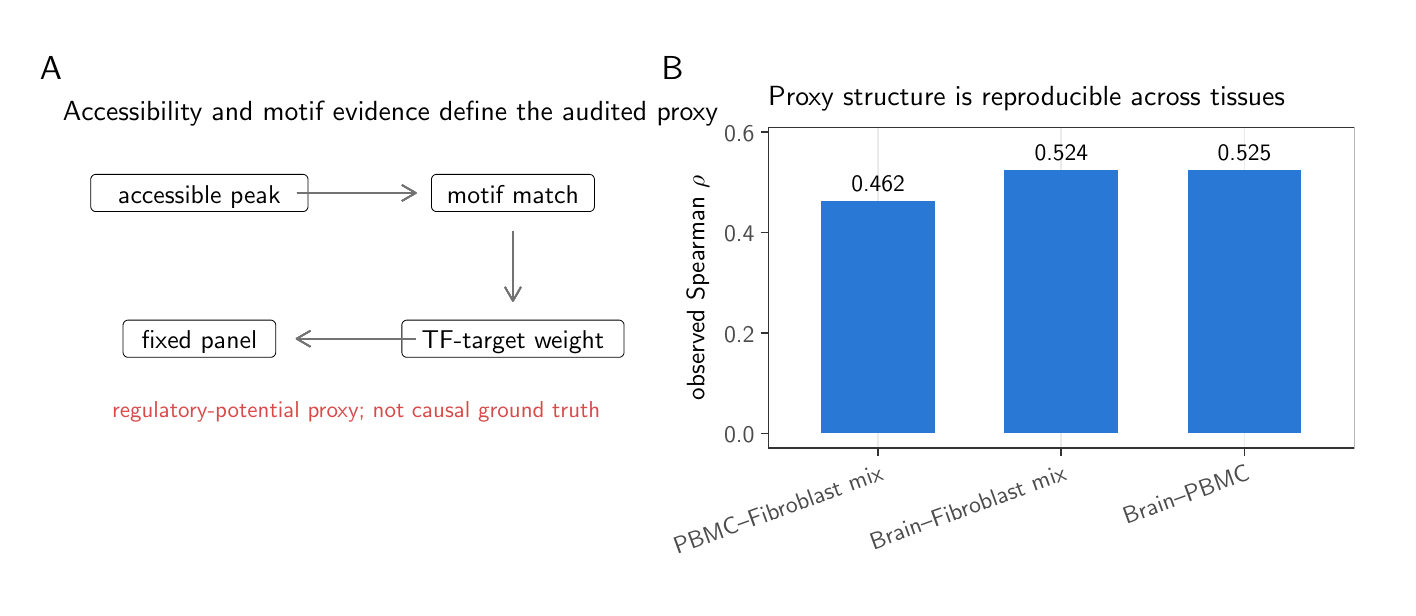
\begin{tikzpicture}[x=1pt,y=1pt]
\definecolor{fillColor}{RGB}{255,255,255}
\path[use as bounding box,fill=fillColor,fill opacity=0.00] (0,0) rectangle (491.44,202.36);
\begin{scope}
\path[clip] (  0.00,  0.00) rectangle (491.44,202.36);
\definecolor{drawColor}{RGB}{255,255,255}
\definecolor{fillColor}{RGB}{255,255,255}

\path[draw=drawColor,line width= 0.6pt,line join=round,line cap=round,fill=fillColor] ( -0.00, -0.00) rectangle (491.44,202.36);
\end{scope}
\begin{scope}
\path[clip] (  4.00,  3.00) rectangle (224.64,198.36);

\path[] (  4.00,  3.00) rectangle (224.64,198.36);
\end{scope}
\begin{scope}
\path[clip] (224.64,  3.00) rectangle (485.44,198.36);
\definecolor{drawColor}{RGB}{255,255,255}
\definecolor{fillColor}{RGB}{255,255,255}

\path[draw=drawColor,line width= 0.6pt,line join=round,line cap=round,fill=fillColor] (224.64,  3.00) rectangle (485.44,198.36);
\end{scope}
\begin{scope}
\path[clip] (  0.00,  0.00) rectangle (491.44,202.36);
\definecolor{drawColor}{RGB}{0,0,0}
\definecolor{fillColor}{RGB}{255,255,255}

\path[draw=drawColor,line width= 0.3pt,line join=round,line cap=round,fill=fillColor] ( 24.65,135.91) --
	( 99.45,135.91) --
	( 99.38,135.92) --
	( 99.68,135.93) --
	( 99.97,135.99) --
	(100.25,136.09) --
	(100.50,136.24) --
	(100.73,136.43) --
	(100.93,136.65) --
	(101.09,136.91) --
	(101.21,137.18) --
	(101.28,137.47) --
	(101.30,137.77) --
	(101.30,137.77) --
	(101.30,147.50) --
	(101.30,147.50) --
	(101.28,147.79) --
	(101.21,148.08) --
	(101.09,148.36) --
	(100.93,148.61) --
	(100.73,148.83) --
	(100.50,149.02) --
	(100.25,149.17) --
	( 99.97,149.28) --
	( 99.68,149.33) --
	( 99.45,149.35) --
	( 24.65,149.35) --
	( 24.87,149.33) --
	( 24.58,149.35) --
	( 24.28,149.31) --
	( 23.99,149.23) --
	( 23.73,149.10) --
	( 23.48,148.93) --
	( 23.27,148.73) --
	( 23.09,148.49) --
	( 22.95,148.22) --
	( 22.85,147.94) --
	( 22.81,147.65) --
	( 22.80,147.50) --
	( 22.80,137.77) --
	( 22.81,137.91) --
	( 22.81,137.62) --
	( 22.85,137.32) --
	( 22.95,137.04) --
	( 23.09,136.78) --
	( 23.27,136.54) --
	( 23.48,136.33) --
	( 23.73,136.16) --
	( 23.99,136.03) --
	( 24.28,135.95) --
	( 24.58,135.92) --
	cycle;
\end{scope}
\begin{scope}
\path[clip] (  0.00,  0.00) rectangle (491.44,202.36);
\definecolor{drawColor}{RGB}{0,0,0}

\node[text=drawColor,anchor=base,inner sep=0pt, outer sep=0pt, scale=  0.93] at ( 62.05,139.00) {accessible peak};
\end{scope}
\begin{scope}
\path[clip] (  0.00,  0.00) rectangle (491.44,202.36);
\definecolor{drawColor}{RGB}{0,0,0}
\definecolor{fillColor}{RGB}{255,255,255}

\path[draw=drawColor,line width= 0.3pt,line join=round,line cap=round,fill=fillColor] (147.77,135.91) --
	(202.94,135.91) --
	(202.86,135.92) --
	(203.16,135.93) --
	(203.45,135.99) --
	(203.73,136.09) --
	(203.99,136.24) --
	(204.22,136.43) --
	(204.42,136.65) --
	(204.58,136.91) --
	(204.69,137.18) --
	(204.76,137.47) --
	(204.79,137.77) --
	(204.79,137.77) --
	(204.79,147.50) --
	(204.79,147.50) --
	(204.76,147.79) --
	(204.69,148.08) --
	(204.58,148.36) --
	(204.42,148.61) --
	(204.22,148.83) --
	(203.99,149.02) --
	(203.73,149.17) --
	(203.45,149.28) --
	(203.16,149.33) --
	(202.94,149.35) --
	(147.77,149.35) --
	(148.00,149.33) --
	(147.70,149.35) --
	(147.40,149.31) --
	(147.12,149.23) --
	(146.85,149.10) --
	(146.60,148.93) --
	(146.39,148.73) --
	(146.21,148.49) --
	(146.07,148.22) --
	(145.98,147.94) --
	(145.93,147.65) --
	(145.92,147.50) --
	(145.92,137.77) --
	(145.93,137.91) --
	(145.93,137.62) --
	(145.98,137.32) --
	(146.07,137.04) --
	(146.21,136.78) --
	(146.39,136.54) --
	(146.60,136.33) --
	(146.85,136.16) --
	(147.12,136.03) --
	(147.40,135.95) --
	(147.70,135.92) --
	cycle;
\end{scope}
\begin{scope}
\path[clip] (  0.00,  0.00) rectangle (491.44,202.36);
\definecolor{drawColor}{RGB}{0,0,0}

\node[text=drawColor,anchor=base,inner sep=0pt, outer sep=0pt, scale=  0.93] at (175.36,139.00) {motif match};
\end{scope}
\begin{scope}
\path[clip] (  0.00,  0.00) rectangle (491.44,202.36);
\definecolor{drawColor}{RGB}{0,0,0}
\definecolor{fillColor}{RGB}{255,255,255}

\path[draw=drawColor,line width= 0.3pt,line join=round,line cap=round,fill=fillColor] (137.06, 83.25) --
	(213.65, 83.25) --
	(213.58, 83.25) --
	(213.88, 83.26) --
	(214.17, 83.32) --
	(214.45, 83.43) --
	(214.70, 83.57) --
	(214.93, 83.76) --
	(215.13, 83.99) --
	(215.29, 84.24) --
	(215.41, 84.51) --
	(215.48, 84.80) --
	(215.50, 85.10) --
	(215.50, 85.10) --
	(215.50, 94.83) --
	(215.50, 94.83) --
	(215.48, 95.13) --
	(215.41, 95.42) --
	(215.29, 95.69) --
	(215.13, 95.94) --
	(214.93, 96.16) --
	(214.70, 96.35) --
	(214.45, 96.50) --
	(214.17, 96.61) --
	(213.88, 96.67) --
	(213.65, 96.68) --
	(137.06, 96.68) --
	(137.28, 96.67) --
	(136.98, 96.68) --
	(136.69, 96.64) --
	(136.40, 96.56) --
	(136.13, 96.43) --
	(135.89, 96.26) --
	(135.67, 96.06) --
	(135.49, 95.82) --
	(135.35, 95.56) --
	(135.26, 95.27) --
	(135.21, 94.98) --
	(135.21, 94.83) --
	(135.21, 85.10) --
	(135.21, 85.25) --
	(135.21, 84.95) --
	(135.26, 84.65) --
	(135.35, 84.37) --
	(135.49, 84.11) --
	(135.67, 83.87) --
	(135.89, 83.66) --
	(136.13, 83.49) --
	(136.40, 83.37) --
	(136.69, 83.28) --
	(136.98, 83.25) --
	cycle;
\end{scope}
\begin{scope}
\path[clip] (  0.00,  0.00) rectangle (491.44,202.36);
\definecolor{drawColor}{RGB}{0,0,0}

\node[text=drawColor,anchor=base,inner sep=0pt, outer sep=0pt, scale=  0.93] at (175.36, 86.33) {TF-target weight};
\end{scope}
\begin{scope}
\path[clip] (  0.00,  0.00) rectangle (491.44,202.36);
\definecolor{drawColor}{RGB}{0,0,0}
\definecolor{fillColor}{RGB}{255,255,255}

\path[draw=drawColor,line width= 0.3pt,line join=round,line cap=round,fill=fillColor] ( 36.32, 83.25) --
	( 87.79, 83.25) --
	( 87.71, 83.25) --
	( 88.01, 83.26) --
	( 88.30, 83.32) --
	( 88.58, 83.43) --
	( 88.84, 83.57) --
	( 89.07, 83.76) --
	( 89.27, 83.99) --
	( 89.43, 84.24) --
	( 89.54, 84.51) --
	( 89.61, 84.80) --
	( 89.64, 85.10) --
	( 89.64, 85.10) --
	( 89.64, 94.83) --
	( 89.64, 94.83) --
	( 89.61, 95.13) --
	( 89.54, 95.42) --
	( 89.43, 95.69) --
	( 89.27, 95.94) --
	( 89.07, 96.16) --
	( 88.84, 96.35) --
	( 88.58, 96.50) --
	( 88.30, 96.61) --
	( 88.01, 96.67) --
	( 87.79, 96.68) --
	( 36.32, 96.68) --
	( 36.54, 96.67) --
	( 36.24, 96.68) --
	( 35.95, 96.64) --
	( 35.66, 96.56) --
	( 35.39, 96.43) --
	( 35.14, 96.26) --
	( 34.93, 96.06) --
	( 34.75, 95.82) --
	( 34.61, 95.56) --
	( 34.52, 95.27) --
	( 34.47, 94.98) --
	( 34.46, 94.83) --
	( 34.46, 85.10) --
	( 34.47, 85.25) --
	( 34.47, 84.95) --
	( 34.52, 84.65) --
	( 34.61, 84.37) --
	( 34.75, 84.11) --
	( 34.93, 83.87) --
	( 35.14, 83.66) --
	( 35.39, 83.49) --
	( 35.66, 83.37) --
	( 35.95, 83.28) --
	( 36.24, 83.25) --
	cycle;
\end{scope}
\begin{scope}
\path[clip] (  0.00,  0.00) rectangle (491.44,202.36);
\definecolor{drawColor}{RGB}{0,0,0}

\node[text=drawColor,anchor=base,inner sep=0pt, outer sep=0pt, scale=  0.93] at ( 62.05, 86.33) {fixed panel};
\end{scope}
\begin{scope}
\path[clip] (  0.00,  0.00) rectangle (491.44,202.36);
\definecolor{drawColor}{gray}{0.45}

\path[draw=drawColor,line width= 0.6pt,line join=round] ( 97.18,142.63) -- (140.23,142.63);

\path[draw=drawColor,line width= 0.6pt,line join=round] (135.22,139.74) --
	(140.23,142.63) --
	(135.22,145.52);

\path[draw=drawColor,line width= 0.6pt,line join=round] ( 97.18,142.63) -- (140.23,142.63);

\path[draw=drawColor,line width= 0.6pt,line join=round] (135.22,139.74) --
	(140.23,142.63) --
	(135.22,145.52);

\path[draw=drawColor,line width= 0.6pt,line join=round] ( 97.18,142.63) -- (140.23,142.63);

\path[draw=drawColor,line width= 0.6pt,line join=round] (135.22,139.74) --
	(140.23,142.63) --
	(135.22,145.52);

\path[draw=drawColor,line width= 0.6pt,line join=round] ( 97.18,142.63) -- (140.23,142.63);

\path[draw=drawColor,line width= 0.6pt,line join=round] (135.22,139.74) --
	(140.23,142.63) --
	(135.22,145.52);

\path[draw=drawColor,line width= 0.6pt,line join=round] (175.36,128.94) -- (175.36,103.66);

\path[draw=drawColor,line width= 0.6pt,line join=round] (172.46,108.66) --
	(175.36,103.66) --
	(178.25,108.66);

\path[draw=drawColor,line width= 0.6pt,line join=round] (175.36,128.94) -- (175.36,103.66);

\path[draw=drawColor,line width= 0.6pt,line join=round] (172.46,108.66) --
	(175.36,103.66) --
	(178.25,108.66);

\path[draw=drawColor,line width= 0.6pt,line join=round] (175.36,128.94) -- (175.36,103.66);

\path[draw=drawColor,line width= 0.6pt,line join=round] (172.46,108.66) --
	(175.36,103.66) --
	(178.25,108.66);

\path[draw=drawColor,line width= 0.6pt,line join=round] (175.36,128.94) -- (175.36,103.66);

\path[draw=drawColor,line width= 0.6pt,line join=round] (172.46,108.66) --
	(175.36,103.66) --
	(178.25,108.66);

\path[draw=drawColor,line width= 0.6pt,line join=round] (140.23, 89.96) -- ( 97.18, 89.96);

\path[draw=drawColor,line width= 0.6pt,line join=round] (102.18, 92.85) --
	( 97.18, 89.96) --
	(102.18, 87.07);

\path[draw=drawColor,line width= 0.6pt,line join=round] (140.23, 89.96) -- ( 97.18, 89.96);

\path[draw=drawColor,line width= 0.6pt,line join=round] (102.18, 92.85) --
	( 97.18, 89.96) --
	(102.18, 87.07);

\path[draw=drawColor,line width= 0.6pt,line join=round] (140.23, 89.96) -- ( 97.18, 89.96);

\path[draw=drawColor,line width= 0.6pt,line join=round] (102.18, 92.85) --
	( 97.18, 89.96) --
	(102.18, 87.07);

\path[draw=drawColor,line width= 0.6pt,line join=round] (140.23, 89.96) -- ( 97.18, 89.96);

\path[draw=drawColor,line width= 0.6pt,line join=round] (102.18, 92.85) --
	( 97.18, 89.96) --
	(102.18, 87.07);
\definecolor{drawColor}{RGB}{216,74,74}

\node[text=drawColor,anchor=base,inner sep=0pt, outer sep=0pt, scale=  0.83] at (118.70, 61.45) {regulatory-potential proxy; not causal ground truth};
\end{scope}
\begin{scope}
\path[clip] (  0.00,  0.00) rectangle (491.44,202.36);
\definecolor{drawColor}{RGB}{0,0,0}

\node[text=drawColor,anchor=base west,inner sep=0pt, outer sep=0pt, scale=  1.00] at ( 12.76,168.77) {Accessibility and motif evidence define the audited proxy};
\end{scope}
\begin{scope}
\path[clip] (  0.00,  0.00) rectangle (491.44,202.36);
\definecolor{drawColor}{RGB}{0,0,0}

\node[text=drawColor,anchor=base,inner sep=0pt, outer sep=0pt, scale=  1.20] at (  8.38,183.53) {A};
\end{scope}
\begin{scope}
\path[clip] (267.56, 50.46) rectangle (479.44,166.33);
\definecolor{fillColor}{RGB}{255,255,255}

\path[fill=fillColor] (267.56, 50.46) rectangle (479.44,166.33);
\definecolor{drawColor}{gray}{0.92}

\path[draw=drawColor,line width= 0.6pt,line join=round] (307.29, 50.46) --
	(307.29,166.33);

\path[draw=drawColor,line width= 0.6pt,line join=round] (373.50, 50.46) --
	(373.50,166.33);

\path[draw=drawColor,line width= 0.6pt,line join=round] (439.71, 50.46) --
	(439.71,166.33);
\definecolor{fillColor}{RGB}{42,120,214}

\path[fill=fillColor] (419.18, 55.73) rectangle (460.23,151.05);

\path[fill=fillColor] (352.97, 55.73) rectangle (394.02,150.99);

\path[fill=fillColor] (286.76, 55.73) rectangle (327.81,139.69);
\definecolor{drawColor}{RGB}{0,0,0}

\node[text=drawColor,anchor=base,inner sep=0pt, outer sep=0pt, scale=  0.85] at (439.71,154.38) {0.525};

\node[text=drawColor,anchor=base,inner sep=0pt, outer sep=0pt, scale=  0.85] at (373.50,154.31) {0.524};

\node[text=drawColor,anchor=base,inner sep=0pt, outer sep=0pt, scale=  0.85] at (307.29,143.02) {0.462};
\definecolor{drawColor}{gray}{0.20}

\path[draw=drawColor,line width= 0.6pt,line join=round,line cap=round] (267.56, 50.46) rectangle (479.44,166.33);
\end{scope}
\begin{scope}
\path[clip] (  0.00,  0.00) rectangle (491.44,202.36);
\definecolor{drawColor}{gray}{0.30}

\node[text=drawColor,anchor=base east,inner sep=0pt, outer sep=0pt, scale=  0.86] at (262.61, 52.36) {0.0};

\node[text=drawColor,anchor=base east,inner sep=0pt, outer sep=0pt, scale=  0.86] at (262.61, 88.68) {0.2};

\node[text=drawColor,anchor=base east,inner sep=0pt, outer sep=0pt, scale=  0.86] at (262.61,125.01) {0.4};

\node[text=drawColor,anchor=base east,inner sep=0pt, outer sep=0pt, scale=  0.86] at (262.61,161.33) {0.6};
\end{scope}
\begin{scope}
\path[clip] (  0.00,  0.00) rectangle (491.44,202.36);
\definecolor{drawColor}{gray}{0.20}

\path[draw=drawColor,line width= 0.6pt,line join=round] (264.81, 55.73) --
	(267.56, 55.73);

\path[draw=drawColor,line width= 0.6pt,line join=round] (264.81, 92.05) --
	(267.56, 92.05);

\path[draw=drawColor,line width= 0.6pt,line join=round] (264.81,128.37) --
	(267.56,128.37);

\path[draw=drawColor,line width= 0.6pt,line join=round] (264.81,164.70) --
	(267.56,164.70);
\end{scope}
\begin{scope}
\path[clip] (  0.00,  0.00) rectangle (491.44,202.36);
\definecolor{drawColor}{gray}{0.20}

\path[draw=drawColor,line width= 0.6pt,line join=round] (307.29, 47.71) --
	(307.29, 50.46);

\path[draw=drawColor,line width= 0.6pt,line join=round] (373.50, 47.71) --
	(373.50, 50.46);

\path[draw=drawColor,line width= 0.6pt,line join=round] (439.71, 47.71) --
	(439.71, 50.46);
\end{scope}
\begin{scope}
\path[clip] (  0.00,  0.00) rectangle (491.44,202.36);
\definecolor{drawColor}{gray}{0.30}

\node[text=drawColor,rotate= 20.00,anchor=base east,inner sep=0pt, outer sep=0pt, scale=  0.86] at (309.59, 39.18) {PBMC--Fibroblast mix};

\node[text=drawColor,rotate= 20.00,anchor=base east,inner sep=0pt, outer sep=0pt, scale=  0.86] at (375.80, 39.18) {Brain--Fibroblast mix};

\node[text=drawColor,rotate= 20.00,anchor=base east,inner sep=0pt, outer sep=0pt, scale=  0.86] at (442.01, 39.18) {Brain--PBMC};
\end{scope}
\begin{scope}
\path[clip] (  0.00,  0.00) rectangle (491.44,202.36);
\definecolor{drawColor}{RGB}{0,0,0}

\node[text=drawColor,rotate= 90.00,anchor=base,inner sep=0pt, outer sep=0pt, scale=  0.91] at (244.50,108.40) {observed Spearman $\rho$};
\end{scope}
\begin{scope}
\path[clip] (  0.00,  0.00) rectangle (491.44,202.36);
\definecolor{drawColor}{RGB}{0,0,0}

\node[text=drawColor,anchor=base west,inner sep=0pt, outer sep=0pt, scale=  1.00] at (267.56,174.27) {Proxy structure is reproducible across tissues};
\end{scope}
\begin{scope}
\path[clip] (  0.00,  0.00) rectangle (491.44,202.36);
\definecolor{drawColor}{RGB}{0,0,0}

\node[text=drawColor,anchor=base,inner sep=0pt, outer sep=0pt, scale=  1.20] at (233.02,183.53) {B};
\end{scope}
\end{tikzpicture}
}
\caption{Regulatory-potential proxy and observed reproducibility. (A) The proxy combines accessible
peaks, motif matches, and TF--target linkage on a fixed panel; it is not causal ground truth.
(B) Observed consensus-graph correlations across three tissue datasets.}\label{fig:proxy}
\vspace{0.8em}
\resizebox{0.72\textwidth}{!}{\begin{tabular}{lrrrrrrr}
\toprule
Tissue pair & Obs.\ $\rho$ & Add.\ frac.\ & Resid.\ $\rho$ & $\varphi$ & Edge Jac.\ & Mean row $\rho$ & Shared TFs \\ 
\midrule
Brain--PBMC & $0.5249$ & $0.7543$ & $0.5073$ & $0.5070$ & $0.416$ & $0.4001$ & 446 \\
Brain--Fibroblast mix & $0.5245$ & $0.7771$ & $0.5502$ & $0.5004$ & $0.414$ & $0.4151$ & 446 \\
PBMC--Fibroblast mix & $0.4623$ & $0.6895$ & $0.4117$ & $0.4461$ & $0.374$ & $0.3364$ & 446 \\
\bottomrule
\end{tabular}
}
\captionof{table}{Observed cross-tissue reproducibility of the regulatory-potential proxy. No
confidence interval or new randomization inference is attached to these descriptive comparisons.}
\label{tab:cross}
\end{figure}

\begin{figure}[t]\centering
\resizebox{\textwidth}{!}{% Created by tikzDevice version 0.12.6 on 2026-07-31 11:12:43
% !TEX encoding = UTF-8 Unicode
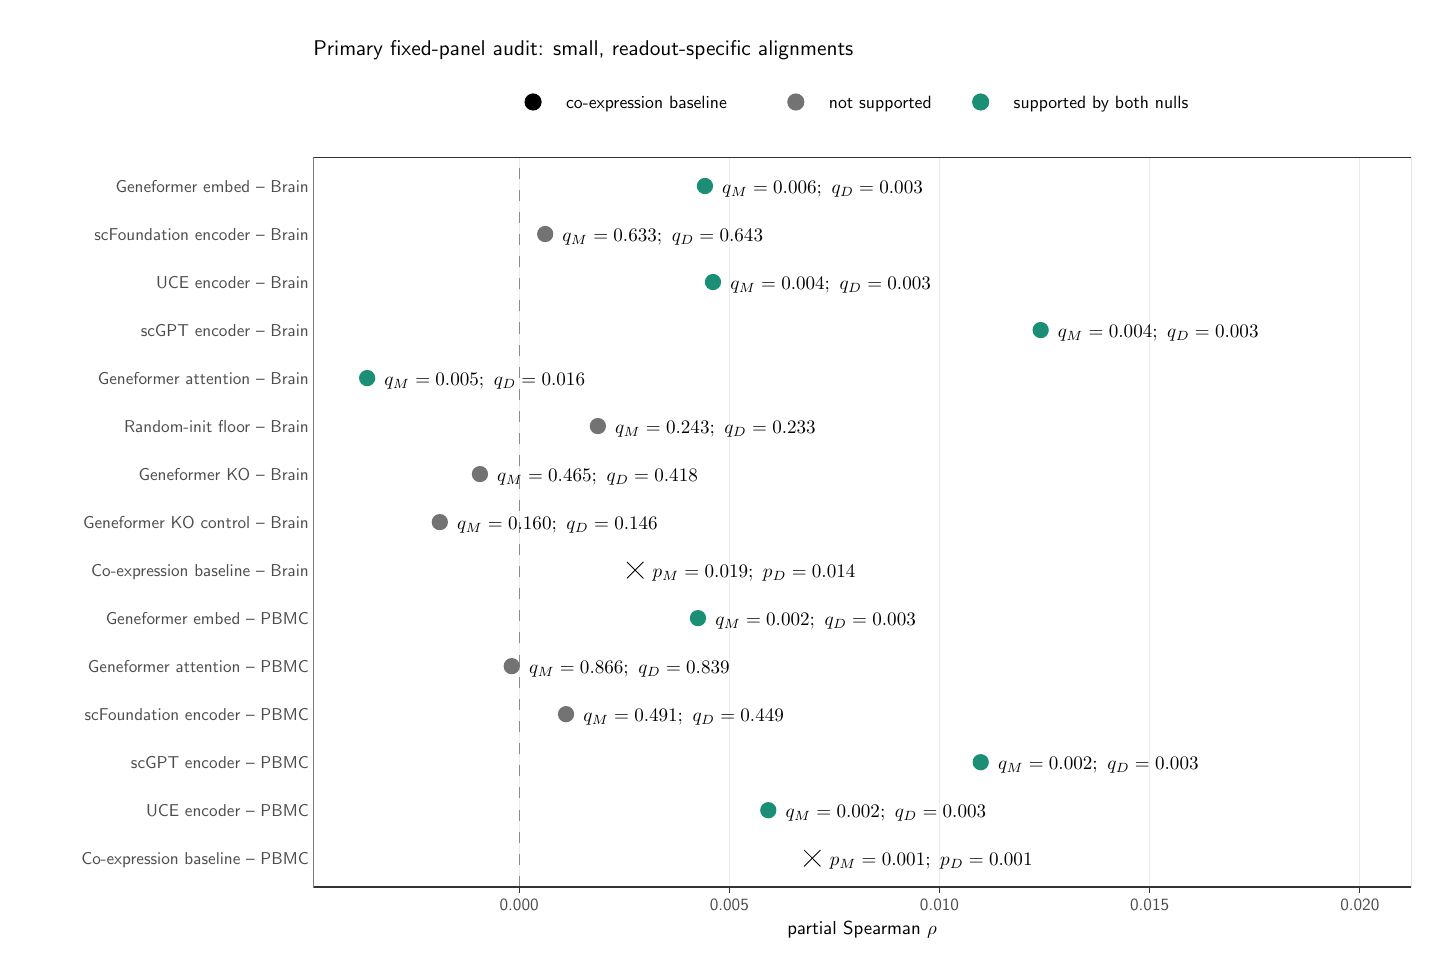
\begin{tikzpicture}[x=1pt,y=1pt]
\definecolor{fillColor}{RGB}{255,255,255}
\path[use as bounding box,fill=fillColor,fill opacity=0.00] (0,0) rectangle (505.89,332.44);
\begin{scope}
\path[clip] (  0.00,  0.00) rectangle (505.89,332.44);
\definecolor{drawColor}{RGB}{255,255,255}
\definecolor{fillColor}{RGB}{255,255,255}

\path[draw=drawColor,line width= 0.4pt,line join=round,line cap=round,fill=fillColor] (  0.00,  0.00) rectangle (505.89,332.44);
\end{scope}
\begin{scope}
\path[clip] (103.20, 21.91) rectangle (499.89,285.63);
\definecolor{fillColor}{RGB}{255,255,255}

\path[fill=fillColor] (103.20, 21.91) rectangle (499.89,285.63);
\definecolor{drawColor}{gray}{0.92}

\path[draw=drawColor,line width= 0.4pt,line join=round] (177.60, 21.91) --
	(177.60,285.63);

\path[draw=drawColor,line width= 0.4pt,line join=round] (253.54, 21.91) --
	(253.54,285.63);

\path[draw=drawColor,line width= 0.4pt,line join=round] (329.48, 21.91) --
	(329.48,285.63);

\path[draw=drawColor,line width= 0.4pt,line join=round] (405.42, 21.91) --
	(405.42,285.63);

\path[draw=drawColor,line width= 0.4pt,line join=round] (481.37, 21.91) --
	(481.37,285.63);
\definecolor{drawColor}{gray}{0.55}

\path[draw=drawColor,line width= 0.4pt,dash pattern=on 4pt off 4pt ,line join=round] (177.60, 21.91) -- (177.60,285.63);
\definecolor{fillColor}{RGB}{27,143,117}

\path[fill=fillColor] (244.73,275.22) circle (  2.94);
\definecolor{fillColor}{gray}{0.45}

\path[fill=fillColor] (187.00,257.87) circle (  2.94);
\definecolor{fillColor}{RGB}{27,143,117}

\path[fill=fillColor] (247.64,240.52) circle (  2.94);

\path[fill=fillColor] (366.04,223.17) circle (  2.94);

\path[fill=fillColor] (122.67,205.82) circle (  2.94);
\definecolor{fillColor}{gray}{0.45}

\path[fill=fillColor] (206.04,188.47) circle (  2.94);

\path[fill=fillColor] (163.42,171.12) circle (  2.94);

\path[fill=fillColor] (148.93,153.77) circle (  2.94);
\definecolor{drawColor}{RGB}{0,0,0}

\path[draw=drawColor,line width= 0.3pt,line join=round,line cap=round] (216.58,133.48) -- (222.45,139.36);

\path[draw=drawColor,line width= 0.3pt,line join=round,line cap=round] (216.58,139.36) -- (222.45,133.48);
\definecolor{fillColor}{RGB}{27,143,117}

\path[fill=fillColor] (242.21,119.07) circle (  2.94);
\definecolor{fillColor}{gray}{0.45}

\path[fill=fillColor] (174.92,101.72) circle (  2.94);

\path[fill=fillColor] (194.53, 84.37) circle (  2.94);
\definecolor{fillColor}{RGB}{27,143,117}

\path[fill=fillColor] (344.38, 67.02) circle (  2.94);

\path[fill=fillColor] (267.62, 49.67) circle (  2.94);

\path[draw=drawColor,line width= 0.3pt,line join=round,line cap=round] (280.59, 29.38) -- (286.46, 35.26);

\path[draw=drawColor,line width= 0.3pt,line join=round,line cap=round] (280.59, 35.26) -- (286.46, 29.38);

\node[text=drawColor,anchor=base west,inner sep=0pt, outer sep=0pt, scale=  0.69] at (250.98,272.55) {$q_M=0.006;\ q_D=0.003$};

\node[text=drawColor,anchor=base west,inner sep=0pt, outer sep=0pt, scale=  0.69] at (193.25,255.20) {$q_M=0.633;\ q_D=0.643$};

\node[text=drawColor,anchor=base west,inner sep=0pt, outer sep=0pt, scale=  0.69] at (253.90,237.85) {$q_M=0.004;\ q_D=0.003$};

\node[text=drawColor,anchor=base west,inner sep=0pt, outer sep=0pt, scale=  0.69] at (372.29,220.50) {$q_M=0.004;\ q_D=0.003$};

\node[text=drawColor,anchor=base west,inner sep=0pt, outer sep=0pt, scale=  0.69] at (128.93,203.15) {$q_M=0.005;\ q_D=0.016$};

\node[text=drawColor,anchor=base west,inner sep=0pt, outer sep=0pt, scale=  0.69] at (212.29,185.80) {$q_M=0.243;\ q_D=0.233$};

\node[text=drawColor,anchor=base west,inner sep=0pt, outer sep=0pt, scale=  0.69] at (169.68,168.45) {$q_M=0.465;\ q_D=0.418$};

\node[text=drawColor,anchor=base west,inner sep=0pt, outer sep=0pt, scale=  0.69] at (155.19,151.10) {$q_M=0.160;\ q_D=0.146$};

\node[text=drawColor,anchor=base west,inner sep=0pt, outer sep=0pt, scale=  0.69] at (225.83,133.75) {$p_M=0.019;\ p_D=0.014$};

\node[text=drawColor,anchor=base west,inner sep=0pt, outer sep=0pt, scale=  0.69] at (248.46,116.40) {$q_M=0.002;\ q_D=0.003$};

\node[text=drawColor,anchor=base west,inner sep=0pt, outer sep=0pt, scale=  0.69] at (181.17, 99.05) {$q_M=0.866;\ q_D=0.839$};

\node[text=drawColor,anchor=base west,inner sep=0pt, outer sep=0pt, scale=  0.69] at (200.78, 81.70) {$q_M=0.491;\ q_D=0.449$};

\node[text=drawColor,anchor=base west,inner sep=0pt, outer sep=0pt, scale=  0.69] at (350.63, 64.35) {$q_M=0.002;\ q_D=0.003$};

\node[text=drawColor,anchor=base west,inner sep=0pt, outer sep=0pt, scale=  0.69] at (273.87, 47.00) {$q_M=0.002;\ q_D=0.003$};

\node[text=drawColor,anchor=base west,inner sep=0pt, outer sep=0pt, scale=  0.69] at (289.85, 29.65) {$p_M=0.001;\ p_D=0.001$};
\definecolor{drawColor}{gray}{0.20}

\path[draw=drawColor,line width= 0.4pt,line join=round,line cap=round] (103.20, 21.91) rectangle (499.89,285.63);
\end{scope}
\begin{scope}
\path[clip] (  0.00,  0.00) rectangle (505.89,332.44);
\definecolor{drawColor}{gray}{0.30}

\node[text=drawColor,anchor=base east,inner sep=0pt, outer sep=0pt, scale=  0.62] at (101.60, 29.91) {Co-expression baseline -- PBMC};

\node[text=drawColor,anchor=base east,inner sep=0pt, outer sep=0pt, scale=  0.62] at (101.60, 47.26) {UCE encoder -- PBMC};

\node[text=drawColor,anchor=base east,inner sep=0pt, outer sep=0pt, scale=  0.62] at (101.60, 64.61) {scGPT encoder -- PBMC};

\node[text=drawColor,anchor=base east,inner sep=0pt, outer sep=0pt, scale=  0.62] at (101.60, 81.96) {scFoundation encoder -- PBMC};

\node[text=drawColor,anchor=base east,inner sep=0pt, outer sep=0pt, scale=  0.62] at (101.60, 99.31) {Geneformer attention -- PBMC};

\node[text=drawColor,anchor=base east,inner sep=0pt, outer sep=0pt, scale=  0.62] at (101.60,116.66) {Geneformer embed -- PBMC};

\node[text=drawColor,anchor=base east,inner sep=0pt, outer sep=0pt, scale=  0.62] at (101.60,134.01) {Co-expression baseline -- Brain};

\node[text=drawColor,anchor=base east,inner sep=0pt, outer sep=0pt, scale=  0.62] at (101.60,151.36) {Geneformer KO control -- Brain};

\node[text=drawColor,anchor=base east,inner sep=0pt, outer sep=0pt, scale=  0.62] at (101.60,168.71) {Geneformer KO -- Brain};

\node[text=drawColor,anchor=base east,inner sep=0pt, outer sep=0pt, scale=  0.62] at (101.60,186.06) {Random-init floor -- Brain};

\node[text=drawColor,anchor=base east,inner sep=0pt, outer sep=0pt, scale=  0.62] at (101.60,203.41) {Geneformer attention -- Brain};

\node[text=drawColor,anchor=base east,inner sep=0pt, outer sep=0pt, scale=  0.62] at (101.60,220.76) {scGPT encoder -- Brain};

\node[text=drawColor,anchor=base east,inner sep=0pt, outer sep=0pt, scale=  0.62] at (101.60,238.11) {UCE encoder -- Brain};

\node[text=drawColor,anchor=base east,inner sep=0pt, outer sep=0pt, scale=  0.62] at (101.60,255.46) {scFoundation encoder -- Brain};

\node[text=drawColor,anchor=base east,inner sep=0pt, outer sep=0pt, scale=  0.62] at (101.60,272.81) {Geneformer embed -- Brain};
\end{scope}
\begin{scope}
\path[clip] (  0.00,  0.00) rectangle (505.89,332.44);
\definecolor{drawColor}{gray}{0.20}

\path[draw=drawColor,line width= 0.4pt,line join=round] (177.60, 19.91) --
	(177.60, 21.91);

\path[draw=drawColor,line width= 0.4pt,line join=round] (253.54, 19.91) --
	(253.54, 21.91);

\path[draw=drawColor,line width= 0.4pt,line join=round] (329.48, 19.91) --
	(329.48, 21.91);

\path[draw=drawColor,line width= 0.4pt,line join=round] (405.42, 19.91) --
	(405.42, 21.91);

\path[draw=drawColor,line width= 0.4pt,line join=round] (481.37, 19.91) --
	(481.37, 21.91);
\end{scope}
\begin{scope}
\path[clip] (  0.00,  0.00) rectangle (505.89,332.44);
\definecolor{drawColor}{gray}{0.30}

\node[text=drawColor,anchor=base,inner sep=0pt, outer sep=0pt, scale=  0.62] at (177.60, 13.49) {0.000};

\node[text=drawColor,anchor=base,inner sep=0pt, outer sep=0pt, scale=  0.62] at (253.54, 13.49) {0.005};

\node[text=drawColor,anchor=base,inner sep=0pt, outer sep=0pt, scale=  0.62] at (329.48, 13.49) {0.010};

\node[text=drawColor,anchor=base,inner sep=0pt, outer sep=0pt, scale=  0.62] at (405.42, 13.49) {0.015};

\node[text=drawColor,anchor=base,inner sep=0pt, outer sep=0pt, scale=  0.62] at (481.37, 13.49) {0.020};
\end{scope}
\begin{scope}
\path[clip] (  0.00,  0.00) rectangle (505.89,332.44);
\definecolor{drawColor}{RGB}{0,0,0}

\node[text=drawColor,anchor=base,inner sep=0pt, outer sep=0pt, scale=  0.68] at (301.55,  4.66) {partial Spearman $\rho$};
\end{scope}
\begin{scope}
\path[clip] (  0.00,  0.00) rectangle (505.89,332.44);
\definecolor{fillColor}{RGB}{255,255,255}

\path[fill=fillColor] (170.67,293.63) rectangle (432.43,317.53);
\end{scope}
\begin{scope}
\path[clip] (  0.00,  0.00) rectangle (505.89,332.44);
\definecolor{fillColor}{RGB}{255,255,255}

\path[fill=fillColor] (174.67,297.63) rectangle (190.57,313.53);
\definecolor{drawColor}{RGB}{0,0,0}
\definecolor{fillColor}{RGB}{0,0,0}

\path[draw=drawColor,line width= 0.3pt,line join=round,line cap=round,fill=fillColor] (182.62,305.58) circle (  2.94);
\end{scope}
\begin{scope}
\path[clip] (  0.00,  0.00) rectangle (505.89,332.44);
\definecolor{fillColor}{RGB}{255,255,255}

\path[fill=fillColor] (269.62,297.63) rectangle (285.52,313.53);
\definecolor{drawColor}{gray}{0.45}
\definecolor{fillColor}{gray}{0.45}

\path[draw=drawColor,line width= 0.3pt,line join=round,line cap=round,fill=fillColor] (277.57,305.58) circle (  2.94);
\end{scope}
\begin{scope}
\path[clip] (  0.00,  0.00) rectangle (505.89,332.44);
\definecolor{fillColor}{RGB}{255,255,255}

\path[fill=fillColor] (336.41,297.63) rectangle (352.31,313.53);
\definecolor{drawColor}{RGB}{27,143,117}
\definecolor{fillColor}{RGB}{27,143,117}

\path[draw=drawColor,line width= 0.3pt,line join=round,line cap=round,fill=fillColor] (344.36,305.58) circle (  2.94);
\end{scope}
\begin{scope}
\path[clip] (  0.00,  0.00) rectangle (505.89,332.44);
\definecolor{drawColor}{RGB}{0,0,0}

\node[text=drawColor,anchor=base west,inner sep=0pt, outer sep=0pt, scale=  0.64] at (194.57,303.10) {co-expression baseline};
\end{scope}
\begin{scope}
\path[clip] (  0.00,  0.00) rectangle (505.89,332.44);
\definecolor{drawColor}{RGB}{0,0,0}

\node[text=drawColor,anchor=base west,inner sep=0pt, outer sep=0pt, scale=  0.64] at (289.52,303.10) {not supported};
\end{scope}
\begin{scope}
\path[clip] (  0.00,  0.00) rectangle (505.89,332.44);
\definecolor{drawColor}{RGB}{0,0,0}

\node[text=drawColor,anchor=base west,inner sep=0pt, outer sep=0pt, scale=  0.64] at (356.31,303.10) {supported by both nulls};
\end{scope}
\begin{scope}
\path[clip] (  0.00,  0.00) rectangle (505.89,332.44);
\definecolor{drawColor}{RGB}{0,0,0}

\node[text=drawColor,anchor=base west,inner sep=0pt, outer sep=0pt, scale=  0.77] at (103.20,322.41) {Primary fixed-panel audit: small, readout-specific alignments};
\end{scope}
\end{tikzpicture}
}
\caption{Primary full-confound fixed-panel audit. Points are observed partial Spearman correlations;
labels give BH-adjusted gene-label ($q_M$) and row-shuffle ($q_D$) values within prespecified
families. Green rows are supported by both nulls at $q<0.05$. Crosses mark the co-expression
baseline, tested outside the FM families with uncorrected $p$-values.}\label{fig:primary}
\end{figure}

\begin{figure}[t]\centering
\resizebox{\textwidth}{!}{% Created by tikzDevice version 0.12.6 on 2026-07-31 11:12:44
% !TEX encoding = UTF-8 Unicode
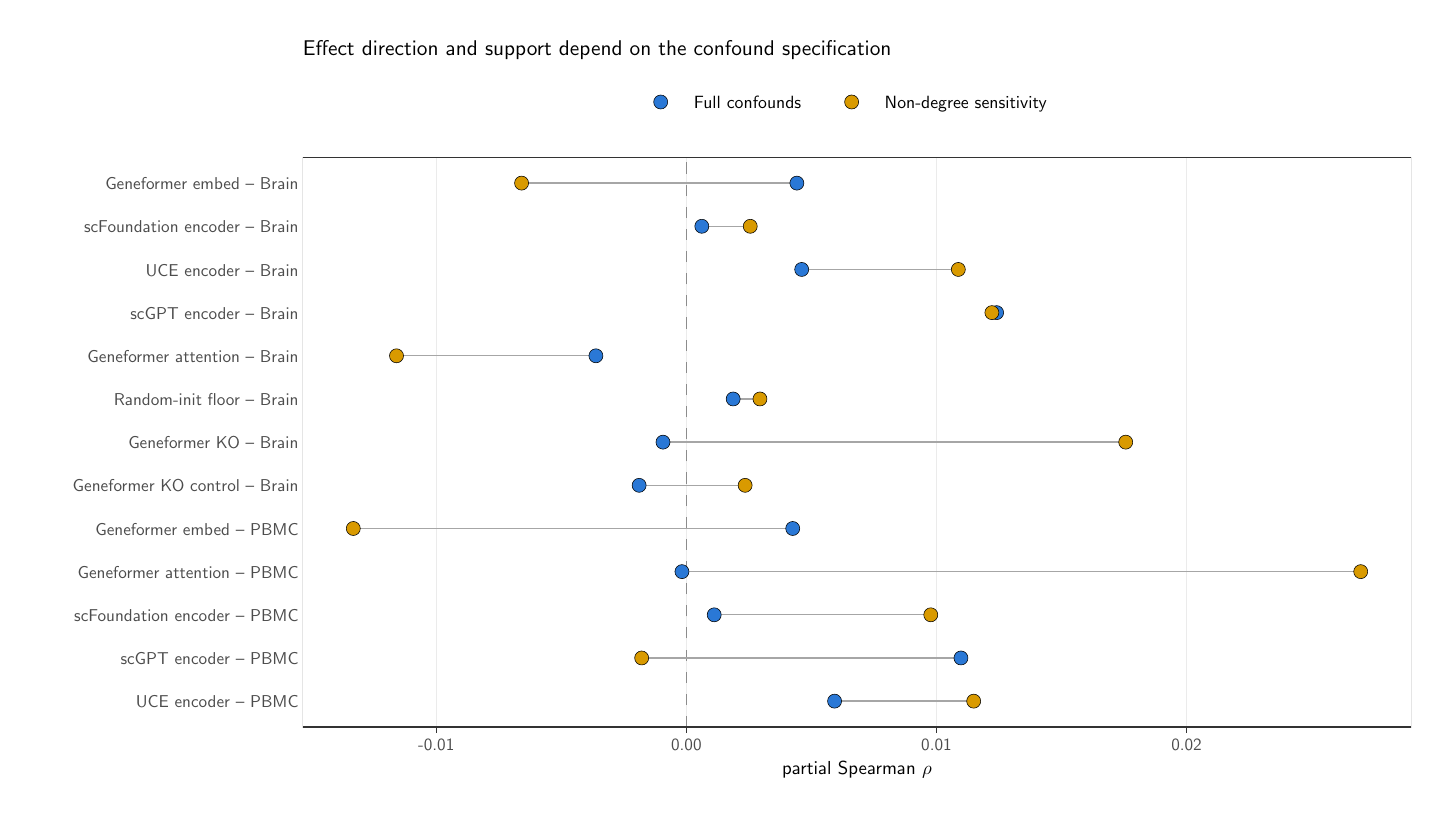
\begin{tikzpicture}[x=1pt,y=1pt]
\definecolor{fillColor}{RGB}{255,255,255}
\path[use as bounding box,fill=fillColor,fill opacity=0.00] (0,0) rectangle (505.89,274.63);
\begin{scope}
\path[clip] (  0.00,  0.00) rectangle (505.89,274.63);
\definecolor{drawColor}{RGB}{255,255,255}
\definecolor{fillColor}{RGB}{255,255,255}

\path[draw=drawColor,line width= 0.4pt,line join=round,line cap=round,fill=fillColor] (  0.00,  0.00) rectangle (505.89,274.63);
\end{scope}
\begin{scope}
\path[clip] ( 99.45, 21.91) rectangle (499.89,227.82);
\definecolor{fillColor}{RGB}{255,255,255}

\path[fill=fillColor] ( 99.45, 21.91) rectangle (499.89,227.82);
\definecolor{drawColor}{gray}{0.92}

\path[draw=drawColor,line width= 0.4pt,line join=round] (147.63, 21.91) --
	(147.63,227.82);

\path[draw=drawColor,line width= 0.4pt,line join=round] (238.01, 21.91) --
	(238.01,227.82);

\path[draw=drawColor,line width= 0.4pt,line join=round] (328.38, 21.91) --
	(328.38,227.82);

\path[draw=drawColor,line width= 0.4pt,line join=round] (418.75, 21.91) --
	(418.75,227.82);
\definecolor{drawColor}{gray}{0.55}

\path[draw=drawColor,line width= 0.4pt,dash pattern=on 4pt off 4pt ,line join=round] (238.01, 21.91) -- (238.01,227.82);
\definecolor{drawColor}{gray}{0.65}

\path[draw=drawColor,line width= 0.5pt,line join=round] (291.57, 31.27) --
	(341.84, 31.27);

\path[draw=drawColor,line width= 0.5pt,line join=round] (221.87, 46.87) --
	(337.24, 46.87);

\path[draw=drawColor,line width= 0.5pt,line join=round] (248.08, 62.47) --
	(326.33, 62.47);

\path[draw=drawColor,line width= 0.5pt,line join=round] (236.42, 78.07) --
	(481.69, 78.07);

\path[draw=drawColor,line width= 0.5pt,line join=round] (117.66, 93.66) --
	(276.45, 93.66);

\path[draw=drawColor,line width= 0.5pt,line join=round] (220.95,109.26) --
	(259.25,109.26);

\path[draw=drawColor,line width= 0.5pt,line join=round] (229.57,124.86) --
	(396.77,124.86);

\path[draw=drawColor,line width= 0.5pt,line join=round] (254.93,140.46) --
	(264.61,140.46);

\path[draw=drawColor,line width= 0.5pt,line join=round] (133.28,156.06) --
	(205.33,156.06);

\path[draw=drawColor,line width= 0.5pt,line join=round] (348.41,171.66) --
	(350.13,171.66);

\path[draw=drawColor,line width= 0.5pt,line join=round] (279.69,187.26) --
	(336.29,187.26);

\path[draw=drawColor,line width= 0.5pt,line join=round] (243.60,202.86) --
	(261.10,202.86);

\path[draw=drawColor,line width= 0.5pt,line join=round] (178.47,218.46) --
	(277.95,218.46);
\definecolor{drawColor}{RGB}{0,0,0}
\definecolor{fillColor}{RGB}{42,120,214}

\path[draw=drawColor,line width= 0.2pt,line join=round,line cap=round,fill=fillColor] (277.95,218.46) circle (  2.53);
\definecolor{fillColor}{RGB}{217,154,0}

\path[draw=drawColor,line width= 0.2pt,line join=round,line cap=round,fill=fillColor] (178.47,218.46) circle (  2.53);
\definecolor{fillColor}{RGB}{42,120,214}

\path[draw=drawColor,line width= 0.2pt,line join=round,line cap=round,fill=fillColor] (243.60,202.86) circle (  2.53);
\definecolor{fillColor}{RGB}{217,154,0}

\path[draw=drawColor,line width= 0.2pt,line join=round,line cap=round,fill=fillColor] (261.10,202.86) circle (  2.53);
\definecolor{fillColor}{RGB}{42,120,214}

\path[draw=drawColor,line width= 0.2pt,line join=round,line cap=round,fill=fillColor] (279.69,187.26) circle (  2.53);
\definecolor{fillColor}{RGB}{217,154,0}

\path[draw=drawColor,line width= 0.2pt,line join=round,line cap=round,fill=fillColor] (336.29,187.26) circle (  2.53);
\definecolor{fillColor}{RGB}{42,120,214}

\path[draw=drawColor,line width= 0.2pt,line join=round,line cap=round,fill=fillColor] (350.13,171.66) circle (  2.53);
\definecolor{fillColor}{RGB}{217,154,0}

\path[draw=drawColor,line width= 0.2pt,line join=round,line cap=round,fill=fillColor] (348.41,171.66) circle (  2.53);
\definecolor{fillColor}{RGB}{42,120,214}

\path[draw=drawColor,line width= 0.2pt,line join=round,line cap=round,fill=fillColor] (205.33,156.06) circle (  2.53);
\definecolor{fillColor}{RGB}{217,154,0}

\path[draw=drawColor,line width= 0.2pt,line join=round,line cap=round,fill=fillColor] (133.28,156.06) circle (  2.53);
\definecolor{fillColor}{RGB}{42,120,214}

\path[draw=drawColor,line width= 0.2pt,line join=round,line cap=round,fill=fillColor] (254.93,140.46) circle (  2.53);
\definecolor{fillColor}{RGB}{217,154,0}

\path[draw=drawColor,line width= 0.2pt,line join=round,line cap=round,fill=fillColor] (264.61,140.46) circle (  2.53);
\definecolor{fillColor}{RGB}{42,120,214}

\path[draw=drawColor,line width= 0.2pt,line join=round,line cap=round,fill=fillColor] (229.57,124.86) circle (  2.53);
\definecolor{fillColor}{RGB}{217,154,0}

\path[draw=drawColor,line width= 0.2pt,line join=round,line cap=round,fill=fillColor] (396.77,124.86) circle (  2.53);
\definecolor{fillColor}{RGB}{42,120,214}

\path[draw=drawColor,line width= 0.2pt,line join=round,line cap=round,fill=fillColor] (220.95,109.26) circle (  2.53);
\definecolor{fillColor}{RGB}{217,154,0}

\path[draw=drawColor,line width= 0.2pt,line join=round,line cap=round,fill=fillColor] (259.25,109.26) circle (  2.53);
\definecolor{fillColor}{RGB}{42,120,214}

\path[draw=drawColor,line width= 0.2pt,line join=round,line cap=round,fill=fillColor] (276.45, 93.66) circle (  2.53);
\definecolor{fillColor}{RGB}{217,154,0}

\path[draw=drawColor,line width= 0.2pt,line join=round,line cap=round,fill=fillColor] (117.66, 93.66) circle (  2.53);
\definecolor{fillColor}{RGB}{42,120,214}

\path[draw=drawColor,line width= 0.2pt,line join=round,line cap=round,fill=fillColor] (236.42, 78.07) circle (  2.53);
\definecolor{fillColor}{RGB}{217,154,0}

\path[draw=drawColor,line width= 0.2pt,line join=round,line cap=round,fill=fillColor] (481.69, 78.07) circle (  2.53);
\definecolor{fillColor}{RGB}{42,120,214}

\path[draw=drawColor,line width= 0.2pt,line join=round,line cap=round,fill=fillColor] (248.08, 62.47) circle (  2.53);
\definecolor{fillColor}{RGB}{217,154,0}

\path[draw=drawColor,line width= 0.2pt,line join=round,line cap=round,fill=fillColor] (326.33, 62.47) circle (  2.53);
\definecolor{fillColor}{RGB}{42,120,214}

\path[draw=drawColor,line width= 0.2pt,line join=round,line cap=round,fill=fillColor] (337.24, 46.87) circle (  2.53);
\definecolor{fillColor}{RGB}{217,154,0}

\path[draw=drawColor,line width= 0.2pt,line join=round,line cap=round,fill=fillColor] (221.87, 46.87) circle (  2.53);
\definecolor{fillColor}{RGB}{42,120,214}

\path[draw=drawColor,line width= 0.2pt,line join=round,line cap=round,fill=fillColor] (291.57, 31.27) circle (  2.53);
\definecolor{fillColor}{RGB}{217,154,0}

\path[draw=drawColor,line width= 0.2pt,line join=round,line cap=round,fill=fillColor] (341.84, 31.27) circle (  2.53);
\definecolor{drawColor}{gray}{0.20}

\path[draw=drawColor,line width= 0.4pt,line join=round,line cap=round] ( 99.45, 21.91) rectangle (499.89,227.82);
\end{scope}
\begin{scope}
\path[clip] (  0.00,  0.00) rectangle (505.89,274.63);
\definecolor{drawColor}{gray}{0.30}

\node[text=drawColor,anchor=base east,inner sep=0pt, outer sep=0pt, scale=  0.62] at ( 97.85, 28.86) {UCE encoder -- PBMC};

\node[text=drawColor,anchor=base east,inner sep=0pt, outer sep=0pt, scale=  0.62] at ( 97.85, 44.46) {scGPT encoder -- PBMC};

\node[text=drawColor,anchor=base east,inner sep=0pt, outer sep=0pt, scale=  0.62] at ( 97.85, 60.06) {scFoundation encoder -- PBMC};

\node[text=drawColor,anchor=base east,inner sep=0pt, outer sep=0pt, scale=  0.62] at ( 97.85, 75.65) {Geneformer attention -- PBMC};

\node[text=drawColor,anchor=base east,inner sep=0pt, outer sep=0pt, scale=  0.62] at ( 97.85, 91.25) {Geneformer embed -- PBMC};

\node[text=drawColor,anchor=base east,inner sep=0pt, outer sep=0pt, scale=  0.62] at ( 97.85,106.85) {Geneformer KO control -- Brain};

\node[text=drawColor,anchor=base east,inner sep=0pt, outer sep=0pt, scale=  0.62] at ( 97.85,122.45) {Geneformer KO -- Brain};

\node[text=drawColor,anchor=base east,inner sep=0pt, outer sep=0pt, scale=  0.62] at ( 97.85,138.05) {Random-init floor -- Brain};

\node[text=drawColor,anchor=base east,inner sep=0pt, outer sep=0pt, scale=  0.62] at ( 97.85,153.65) {Geneformer attention -- Brain};

\node[text=drawColor,anchor=base east,inner sep=0pt, outer sep=0pt, scale=  0.62] at ( 97.85,169.25) {scGPT encoder -- Brain};

\node[text=drawColor,anchor=base east,inner sep=0pt, outer sep=0pt, scale=  0.62] at ( 97.85,184.85) {UCE encoder -- Brain};

\node[text=drawColor,anchor=base east,inner sep=0pt, outer sep=0pt, scale=  0.62] at ( 97.85,200.45) {scFoundation encoder -- Brain};

\node[text=drawColor,anchor=base east,inner sep=0pt, outer sep=0pt, scale=  0.62] at ( 97.85,216.04) {Geneformer embed -- Brain};
\end{scope}
\begin{scope}
\path[clip] (  0.00,  0.00) rectangle (505.89,274.63);
\definecolor{drawColor}{gray}{0.20}

\path[draw=drawColor,line width= 0.4pt,line join=round] (147.63, 19.91) --
	(147.63, 21.91);

\path[draw=drawColor,line width= 0.4pt,line join=round] (238.01, 19.91) --
	(238.01, 21.91);

\path[draw=drawColor,line width= 0.4pt,line join=round] (328.38, 19.91) --
	(328.38, 21.91);

\path[draw=drawColor,line width= 0.4pt,line join=round] (418.75, 19.91) --
	(418.75, 21.91);
\end{scope}
\begin{scope}
\path[clip] (  0.00,  0.00) rectangle (505.89,274.63);
\definecolor{drawColor}{gray}{0.30}

\node[text=drawColor,anchor=base,inner sep=0pt, outer sep=0pt, scale=  0.62] at (147.63, 13.49) {-0.01};

\node[text=drawColor,anchor=base,inner sep=0pt, outer sep=0pt, scale=  0.62] at (238.01, 13.49) {0.00};

\node[text=drawColor,anchor=base,inner sep=0pt, outer sep=0pt, scale=  0.62] at (328.38, 13.49) {0.01};

\node[text=drawColor,anchor=base,inner sep=0pt, outer sep=0pt, scale=  0.62] at (418.75, 13.49) {0.02};
\end{scope}
\begin{scope}
\path[clip] (  0.00,  0.00) rectangle (505.89,274.63);
\definecolor{drawColor}{RGB}{0,0,0}

\node[text=drawColor,anchor=base,inner sep=0pt, outer sep=0pt, scale=  0.68] at (299.67,  4.66) {partial Spearman $\rho$};
\end{scope}
\begin{scope}
\path[clip] (  0.00,  0.00) rectangle (505.89,274.63);
\definecolor{fillColor}{RGB}{255,255,255}

\path[fill=fillColor] (216.79,235.82) rectangle (382.56,259.71);
\end{scope}
\begin{scope}
\path[clip] (  0.00,  0.00) rectangle (505.89,274.63);
\definecolor{fillColor}{RGB}{255,255,255}

\path[fill=fillColor] (220.79,239.82) rectangle (236.69,255.71);
\definecolor{drawColor}{RGB}{0,0,0}
\definecolor{fillColor}{RGB}{42,120,214}

\path[draw=drawColor,line width= 0.2pt,line join=round,line cap=round,fill=fillColor] (228.74,247.77) circle (  2.53);
\end{scope}
\begin{scope}
\path[clip] (  0.00,  0.00) rectangle (505.89,274.63);
\definecolor{fillColor}{RGB}{255,255,255}

\path[fill=fillColor] (289.79,239.82) rectangle (305.69,255.71);
\definecolor{drawColor}{RGB}{0,0,0}
\definecolor{fillColor}{RGB}{217,154,0}

\path[draw=drawColor,line width= 0.2pt,line join=round,line cap=round,fill=fillColor] (297.74,247.77) circle (  2.53);
\end{scope}
\begin{scope}
\path[clip] (  0.00,  0.00) rectangle (505.89,274.63);
\definecolor{drawColor}{RGB}{0,0,0}

\node[text=drawColor,anchor=base west,inner sep=0pt, outer sep=0pt, scale=  0.64] at (240.69,245.28) {Full confounds};
\end{scope}
\begin{scope}
\path[clip] (  0.00,  0.00) rectangle (505.89,274.63);
\definecolor{drawColor}{RGB}{0,0,0}

\node[text=drawColor,anchor=base west,inner sep=0pt, outer sep=0pt, scale=  0.64] at (309.69,245.28) {Non-degree sensitivity};
\end{scope}
\begin{scope}
\path[clip] (  0.00,  0.00) rectangle (505.89,274.63);
\definecolor{drawColor}{RGB}{0,0,0}

\node[text=drawColor,anchor=base west,inner sep=0pt, outer sep=0pt, scale=  0.77] at ( 99.45,264.60) {Effect direction and support depend on the confound specification};
\end{scope}
\end{tikzpicture}
}
\caption{Confound-specification sensitivity. Full and non-degree estimates are joined within each
model/readout and tissue. The non-degree results are secondary and show null-dependent support.}
\label{fig:spec}
\end{figure}

\begin{figure}[t]\centering
\resizebox{0.85\textwidth}{!}{% Created by tikzDevice version 0.12.6 on 2026-08-01 04:31:25
% !TEX encoding = UTF-8 Unicode
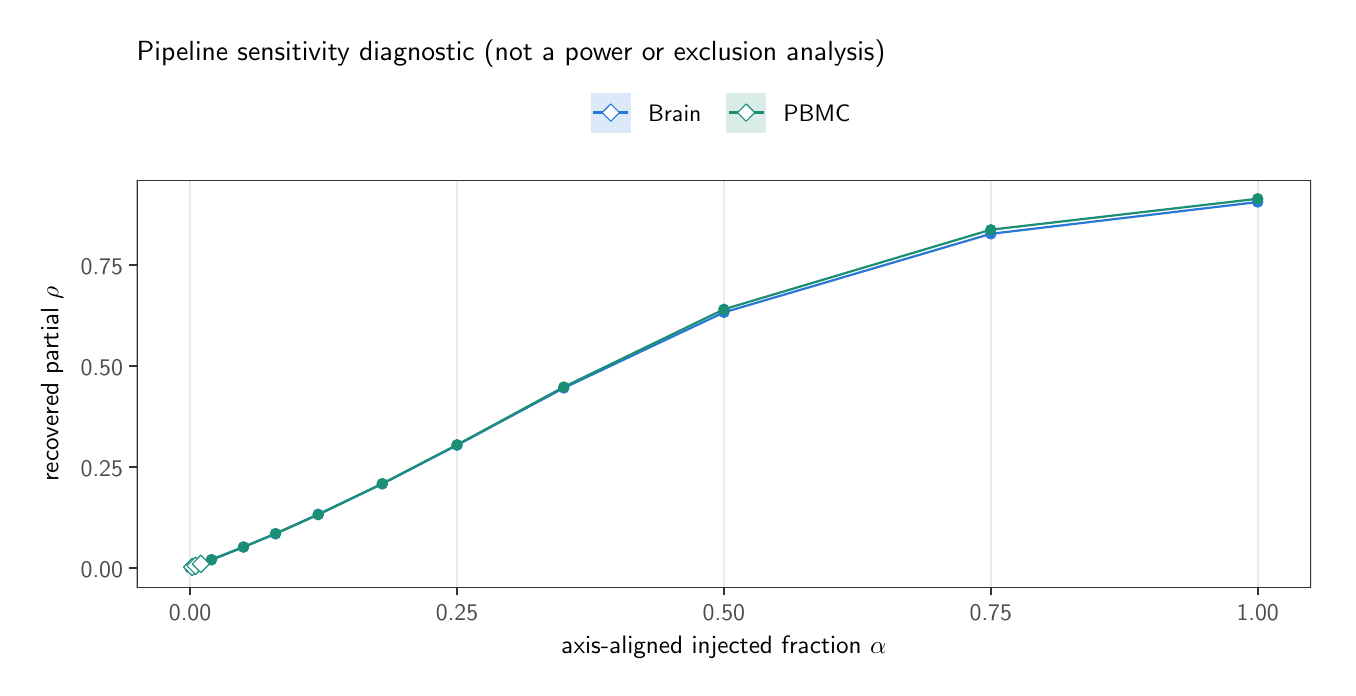
\begin{tikzpicture}[x=1pt,y=1pt]
\definecolor{fillColor}{RGB}{255,255,255}
\path[use as bounding box,fill=fillColor,fill opacity=0.00] (0,0) rectangle (469.75,231.26);
\begin{scope}
\path[clip] (  0.00,  0.00) rectangle (469.75,231.26);
\definecolor{drawColor}{RGB}{255,255,255}
\definecolor{fillColor}{RGB}{255,255,255}

\path[draw=drawColor,line width= 0.6pt,line join=round,line cap=round,fill=fillColor] (  0.00, -0.00) rectangle (469.76,231.26);
\end{scope}
\begin{scope}
\path[clip] ( 39.41, 28.85) rectangle (463.76,176.13);
\definecolor{fillColor}{RGB}{255,255,255}

\path[fill=fillColor] ( 39.41, 28.85) rectangle (463.75,176.13);
\definecolor{drawColor}{gray}{0.92}

\path[draw=drawColor,line width= 0.6pt,line join=round] ( 58.70, 28.85) --
	( 58.70,176.13);

\path[draw=drawColor,line width= 0.6pt,line join=round] (155.14, 28.85) --
	(155.14,176.13);

\path[draw=drawColor,line width= 0.6pt,line join=round] (251.58, 28.85) --
	(251.58,176.13);

\path[draw=drawColor,line width= 0.6pt,line join=round] (348.02, 28.85) --
	(348.02,176.13);

\path[draw=drawColor,line width= 0.6pt,line join=round] (444.47, 28.85) --
	(444.47,176.13);
\definecolor{fillColor}{RGB}{42,120,214}

\path[fill=fillColor,fill opacity=0.16] ( 58.70, 36.52) --
	( 66.41, 39.31) --
	( 77.99, 43.92) --
	( 89.56, 48.76) --
	(104.99, 55.93) --
	(128.14, 66.86) --
	(155.14, 80.71) --
	(193.72,101.33) --
	(251.58,128.58) --
	(348.02,156.80) --
	(444.47,168.25) --
	(444.47,168.25) --
	(348.02,156.72) --
	(251.58,128.27) --
	(193.72,100.80) --
	(155.14, 79.74) --
	(128.14, 66.07) --
	(104.99, 54.98) --
	( 89.56, 48.00) --
	( 77.99, 43.13) --
	( 66.41, 38.63) --
	( 58.70, 35.69) --
	cycle;

\path[] ( 58.70, 36.52) --
	( 66.41, 39.31) --
	( 77.99, 43.92) --
	( 89.56, 48.76) --
	(104.99, 55.93) --
	(128.14, 66.86) --
	(155.14, 80.71) --
	(193.72,101.33) --
	(251.58,128.58) --
	(348.02,156.80) --
	(444.47,168.25);

\path[] (444.47,168.25) --
	(348.02,156.72) --
	(251.58,128.27) --
	(193.72,100.80) --
	(155.14, 79.74) --
	(128.14, 66.07) --
	(104.99, 54.98) --
	( 89.56, 48.00) --
	( 77.99, 43.13) --
	( 66.41, 38.63) --
	( 58.70, 35.69);
\definecolor{fillColor}{RGB}{27,143,117}

\path[fill=fillColor,fill opacity=0.16] ( 58.70, 36.62) --
	( 66.41, 39.65) --
	( 77.99, 44.06) --
	( 89.56, 48.85) --
	(104.99, 55.55) --
	(128.14, 66.93) --
	(155.14, 80.82) --
	(193.72,101.77) --
	(251.58,129.55) --
	(348.02,158.28) --
	(444.47,169.43) --
	(444.47,169.43) --
	(348.02,158.22) --
	(251.58,129.39) --
	(193.72,101.08) --
	(155.14, 80.23) --
	(128.14, 66.12) --
	(104.99, 54.85) --
	( 89.56, 48.11) --
	( 77.99, 43.16) --
	( 66.41, 38.48) --
	( 58.70, 35.54) --
	cycle;

\path[] ( 58.70, 36.62) --
	( 66.41, 39.65) --
	( 77.99, 44.06) --
	( 89.56, 48.85) --
	(104.99, 55.55) --
	(128.14, 66.93) --
	(155.14, 80.82) --
	(193.72,101.77) --
	(251.58,129.55) --
	(348.02,158.28) --
	(444.47,169.43);

\path[] (444.47,169.43) --
	(348.02,158.22) --
	(251.58,129.39) --
	(193.72,101.08) --
	(155.14, 80.23) --
	(128.14, 66.12) --
	(104.99, 54.85) --
	( 89.56, 48.11) --
	( 77.99, 43.16) --
	( 66.41, 38.48) --
	( 58.70, 35.54);
\definecolor{drawColor}{RGB}{42,120,214}

\path[draw=drawColor,line width= 0.8pt,line join=round] ( 58.70, 36.07) --
	( 66.41, 38.99) --
	( 77.99, 43.57) --
	( 89.56, 48.38) --
	(104.99, 55.43) --
	(128.14, 66.42) --
	(155.14, 80.41) --
	(193.72,101.06) --
	(251.58,128.38) --
	(348.02,156.76) --
	(444.47,168.25);
\definecolor{drawColor}{RGB}{27,143,117}

\path[draw=drawColor,line width= 0.8pt,line join=round] ( 58.70, 36.17) --
	( 66.41, 39.01) --
	( 77.99, 43.61) --
	( 89.56, 48.43) --
	(104.99, 55.28) --
	(128.14, 66.48) --
	(155.14, 80.53) --
	(193.72,101.42) --
	(251.58,129.49) --
	(348.02,158.25) --
	(444.47,169.43);
\definecolor{drawColor}{RGB}{42,120,214}
\definecolor{fillColor}{RGB}{42,120,214}

\path[draw=drawColor,line width= 0.4pt,line join=round,line cap=round,fill=fillColor] ( 58.70, 36.07) circle (  1.86);

\path[draw=drawColor,line width= 0.4pt,line join=round,line cap=round,fill=fillColor] ( 66.41, 38.99) circle (  1.86);

\path[draw=drawColor,line width= 0.4pt,line join=round,line cap=round,fill=fillColor] ( 77.99, 43.57) circle (  1.86);

\path[draw=drawColor,line width= 0.4pt,line join=round,line cap=round,fill=fillColor] ( 89.56, 48.38) circle (  1.86);

\path[draw=drawColor,line width= 0.4pt,line join=round,line cap=round,fill=fillColor] (104.99, 55.43) circle (  1.86);

\path[draw=drawColor,line width= 0.4pt,line join=round,line cap=round,fill=fillColor] (128.14, 66.42) circle (  1.86);

\path[draw=drawColor,line width= 0.4pt,line join=round,line cap=round,fill=fillColor] (155.14, 80.41) circle (  1.86);

\path[draw=drawColor,line width= 0.4pt,line join=round,line cap=round,fill=fillColor] (193.72,101.06) circle (  1.86);

\path[draw=drawColor,line width= 0.4pt,line join=round,line cap=round,fill=fillColor] (251.58,128.38) circle (  1.86);

\path[draw=drawColor,line width= 0.4pt,line join=round,line cap=round,fill=fillColor] (348.02,156.76) circle (  1.86);

\path[draw=drawColor,line width= 0.4pt,line join=round,line cap=round,fill=fillColor] (444.47,168.25) circle (  1.86);
\definecolor{drawColor}{RGB}{27,143,117}
\definecolor{fillColor}{RGB}{27,143,117}

\path[draw=drawColor,line width= 0.4pt,line join=round,line cap=round,fill=fillColor] ( 58.70, 36.17) circle (  1.86);

\path[draw=drawColor,line width= 0.4pt,line join=round,line cap=round,fill=fillColor] ( 66.41, 39.01) circle (  1.86);

\path[draw=drawColor,line width= 0.4pt,line join=round,line cap=round,fill=fillColor] ( 77.99, 43.61) circle (  1.86);

\path[draw=drawColor,line width= 0.4pt,line join=round,line cap=round,fill=fillColor] ( 89.56, 48.43) circle (  1.86);

\path[draw=drawColor,line width= 0.4pt,line join=round,line cap=round,fill=fillColor] (104.99, 55.28) circle (  1.86);

\path[draw=drawColor,line width= 0.4pt,line join=round,line cap=round,fill=fillColor] (128.14, 66.48) circle (  1.86);

\path[draw=drawColor,line width= 0.4pt,line join=round,line cap=round,fill=fillColor] (155.14, 80.53) circle (  1.86);

\path[draw=drawColor,line width= 0.4pt,line join=round,line cap=round,fill=fillColor] (193.72,101.42) circle (  1.86);

\path[draw=drawColor,line width= 0.4pt,line join=round,line cap=round,fill=fillColor] (251.58,129.49) circle (  1.86);

\path[draw=drawColor,line width= 0.4pt,line join=round,line cap=round,fill=fillColor] (348.02,158.25) circle (  1.86);

\path[draw=drawColor,line width= 0.4pt,line join=round,line cap=round,fill=fillColor] (444.47,169.43) circle (  1.86);
\definecolor{drawColor}{RGB}{42,120,214}
\definecolor{fillColor}{RGB}{255,255,255}

\path[draw=drawColor,line width= 0.4pt,line join=round,line cap=round,fill=fillColor] ( 59.47, 33.25) --
	( 62.60, 36.38) --
	( 59.47, 39.51) --
	( 56.34, 36.38) --
	cycle;

\path[draw=drawColor,line width= 0.4pt,line join=round,line cap=round,fill=fillColor] ( 60.63, 33.60) --
	( 63.76, 36.73) --
	( 60.63, 39.86) --
	( 57.50, 36.73) --
	cycle;

\path[draw=drawColor,line width= 0.4pt,line join=round,line cap=round,fill=fillColor] ( 62.56, 34.39) --
	( 65.69, 37.52) --
	( 62.56, 40.65) --
	( 59.43, 37.52) --
	cycle;
\definecolor{drawColor}{RGB}{27,143,117}

\path[draw=drawColor,line width= 0.4pt,line join=round,line cap=round,fill=fillColor] ( 59.47, 33.23) --
	( 62.60, 36.36) --
	( 59.47, 39.49) --
	( 56.34, 36.36) --
	cycle;

\path[draw=drawColor,line width= 0.4pt,line join=round,line cap=round,fill=fillColor] ( 60.63, 33.70) --
	( 63.76, 36.83) --
	( 60.63, 39.96) --
	( 57.50, 36.83) --
	cycle;

\path[draw=drawColor,line width= 0.4pt,line join=round,line cap=round,fill=fillColor] ( 62.56, 34.36) --
	( 65.69, 37.49) --
	( 62.56, 40.62) --
	( 59.43, 37.49) --
	cycle;
\definecolor{drawColor}{gray}{0.20}

\path[draw=drawColor,line width= 0.6pt,line join=round,line cap=round] ( 39.41, 28.85) rectangle (463.75,176.13);
\end{scope}
\begin{scope}
\path[clip] (  0.00,  0.00) rectangle (469.75,231.26);
\definecolor{drawColor}{gray}{0.30}

\node[text=drawColor,anchor=base east,inner sep=0pt, outer sep=0pt, scale=  0.86] at ( 34.46, 32.72) {0.00};

\node[text=drawColor,anchor=base east,inner sep=0pt, outer sep=0pt, scale=  0.86] at ( 34.46, 69.22) {0.25};

\node[text=drawColor,anchor=base east,inner sep=0pt, outer sep=0pt, scale=  0.86] at ( 34.46,105.71) {0.50};

\node[text=drawColor,anchor=base east,inner sep=0pt, outer sep=0pt, scale=  0.86] at ( 34.46,142.21) {0.75};
\end{scope}
\begin{scope}
\path[clip] (  0.00,  0.00) rectangle (469.75,231.26);
\definecolor{drawColor}{gray}{0.20}

\path[draw=drawColor,line width= 0.6pt,line join=round] ( 36.66, 36.09) --
	( 39.41, 36.09);

\path[draw=drawColor,line width= 0.6pt,line join=round] ( 36.66, 72.59) --
	( 39.41, 72.59);

\path[draw=drawColor,line width= 0.6pt,line join=round] ( 36.66,109.08) --
	( 39.41,109.08);

\path[draw=drawColor,line width= 0.6pt,line join=round] ( 36.66,145.58) --
	( 39.41,145.58);
\end{scope}
\begin{scope}
\path[clip] (  0.00,  0.00) rectangle (469.75,231.26);
\definecolor{drawColor}{gray}{0.20}

\path[draw=drawColor,line width= 0.6pt,line join=round] ( 58.70, 26.10) --
	( 58.70, 28.85);

\path[draw=drawColor,line width= 0.6pt,line join=round] (155.14, 26.10) --
	(155.14, 28.85);

\path[draw=drawColor,line width= 0.6pt,line join=round] (251.58, 26.10) --
	(251.58, 28.85);

\path[draw=drawColor,line width= 0.6pt,line join=round] (348.02, 26.10) --
	(348.02, 28.85);

\path[draw=drawColor,line width= 0.6pt,line join=round] (444.47, 26.10) --
	(444.47, 28.85);
\end{scope}
\begin{scope}
\path[clip] (  0.00,  0.00) rectangle (469.75,231.26);
\definecolor{drawColor}{gray}{0.30}

\node[text=drawColor,anchor=base,inner sep=0pt, outer sep=0pt, scale=  0.86] at ( 58.70, 17.16) {0.00};

\node[text=drawColor,anchor=base,inner sep=0pt, outer sep=0pt, scale=  0.86] at (155.14, 17.16) {0.25};

\node[text=drawColor,anchor=base,inner sep=0pt, outer sep=0pt, scale=  0.86] at (251.58, 17.16) {0.50};

\node[text=drawColor,anchor=base,inner sep=0pt, outer sep=0pt, scale=  0.86] at (348.02, 17.16) {0.75};

\node[text=drawColor,anchor=base,inner sep=0pt, outer sep=0pt, scale=  0.86] at (444.47, 17.16) {1.00};
\end{scope}
\begin{scope}
\path[clip] (  0.00,  0.00) rectangle (469.75,231.26);
\definecolor{drawColor}{RGB}{0,0,0}

\node[text=drawColor,anchor=base,inner sep=0pt, outer sep=0pt, scale=  0.91] at (251.58,  5.21) {axis-aligned injected fraction $\alpha$};
\end{scope}
\begin{scope}
\path[clip] (  0.00,  0.00) rectangle (469.75,231.26);
\definecolor{drawColor}{RGB}{0,0,0}

\node[text=drawColor,rotate= 90.00,anchor=base,inner sep=0pt, outer sep=0pt, scale=  0.91] at ( 11.09,102.49) {recovered partial $\rho$};
\end{scope}
\begin{scope}
\path[clip] (  0.00,  0.00) rectangle (469.75,231.26);
\definecolor{fillColor}{RGB}{255,255,255}

\path[fill=fillColor] (197.28,187.13) rectangle (305.88,214.03);
\end{scope}
\begin{scope}
\path[clip] (  0.00,  0.00) rectangle (469.75,231.26);
\definecolor{fillColor}{RGB}{255,255,255}

\path[fill=fillColor] (202.78,192.63) rectangle (218.68,208.53);
\definecolor{fillColor}{RGB}{42,120,214}

\path[fill=fillColor,fill opacity=0.16] (203.50,193.34) rectangle (217.97,207.81);
\definecolor{drawColor}{RGB}{42,120,214}

\path[draw=drawColor,line width= 0.8pt,line join=round] (204.37,200.58) -- (217.09,200.58);
\definecolor{fillColor}{RGB}{42,120,214}

\path[draw=drawColor,line width= 0.4pt,line join=round,line cap=round,fill=fillColor] (210.73,200.58) circle (  1.86);
\definecolor{fillColor}{RGB}{255,255,255}

\path[draw=drawColor,line width= 0.4pt,line join=round,line cap=round,fill=fillColor] (210.73,197.45) --
	(213.86,200.58) --
	(210.73,203.71) --
	(207.60,200.58) --
	cycle;
\end{scope}
\begin{scope}
\path[clip] (  0.00,  0.00) rectangle (469.75,231.26);
\definecolor{fillColor}{RGB}{255,255,255}

\path[fill=fillColor] (251.66,192.63) rectangle (267.56,208.53);
\definecolor{fillColor}{RGB}{27,143,117}

\path[fill=fillColor,fill opacity=0.16] (252.37,193.34) rectangle (266.85,207.81);
\definecolor{drawColor}{RGB}{27,143,117}

\path[draw=drawColor,line width= 0.8pt,line join=round] (253.25,200.58) -- (265.97,200.58);
\definecolor{fillColor}{RGB}{27,143,117}

\path[draw=drawColor,line width= 0.4pt,line join=round,line cap=round,fill=fillColor] (259.61,200.58) circle (  1.86);
\definecolor{fillColor}{RGB}{255,255,255}

\path[draw=drawColor,line width= 0.4pt,line join=round,line cap=round,fill=fillColor] (259.61,197.45) --
	(262.74,200.58) --
	(259.61,203.71) --
	(256.48,200.58) --
	cycle;
\end{scope}
\begin{scope}
\path[clip] (  0.00,  0.00) rectangle (469.75,231.26);
\definecolor{drawColor}{RGB}{0,0,0}

\node[text=drawColor,anchor=base west,inner sep=0pt, outer sep=0pt, scale=  0.86] at (224.18,197.21) {Brain};
\end{scope}
\begin{scope}
\path[clip] (  0.00,  0.00) rectangle (469.75,231.26);
\definecolor{drawColor}{RGB}{0,0,0}

\node[text=drawColor,anchor=base west,inner sep=0pt, outer sep=0pt, scale=  0.86] at (273.06,197.21) {PBMC};
\end{scope}
\begin{scope}
\path[clip] (  0.00,  0.00) rectangle (469.75,231.26);
\definecolor{drawColor}{RGB}{0,0,0}

\node[text=drawColor,anchor=base west,inner sep=0pt, outer sep=0pt, scale=  1.00] at ( 39.41,219.46) {Pipeline sensitivity diagnostic (not a power or exclusion analysis)};
\end{scope}
\end{tikzpicture}
}
\caption{Axis-aligned pipeline-sensitivity diagnostic. Lines show the mean across 30 independent
noise replicates and ribbons show the replicate range. This is not a confidence interval, power
curve, MDE, or exclusion analysis.}\label{fig:sensitivity}
\end{figure}

\begin{figure}[t]\centering
\resizebox{\textwidth}{!}{% Created by tikzDevice version 0.12.6 on 2026-07-31 23:28:08
% !TEX encoding = UTF-8 Unicode
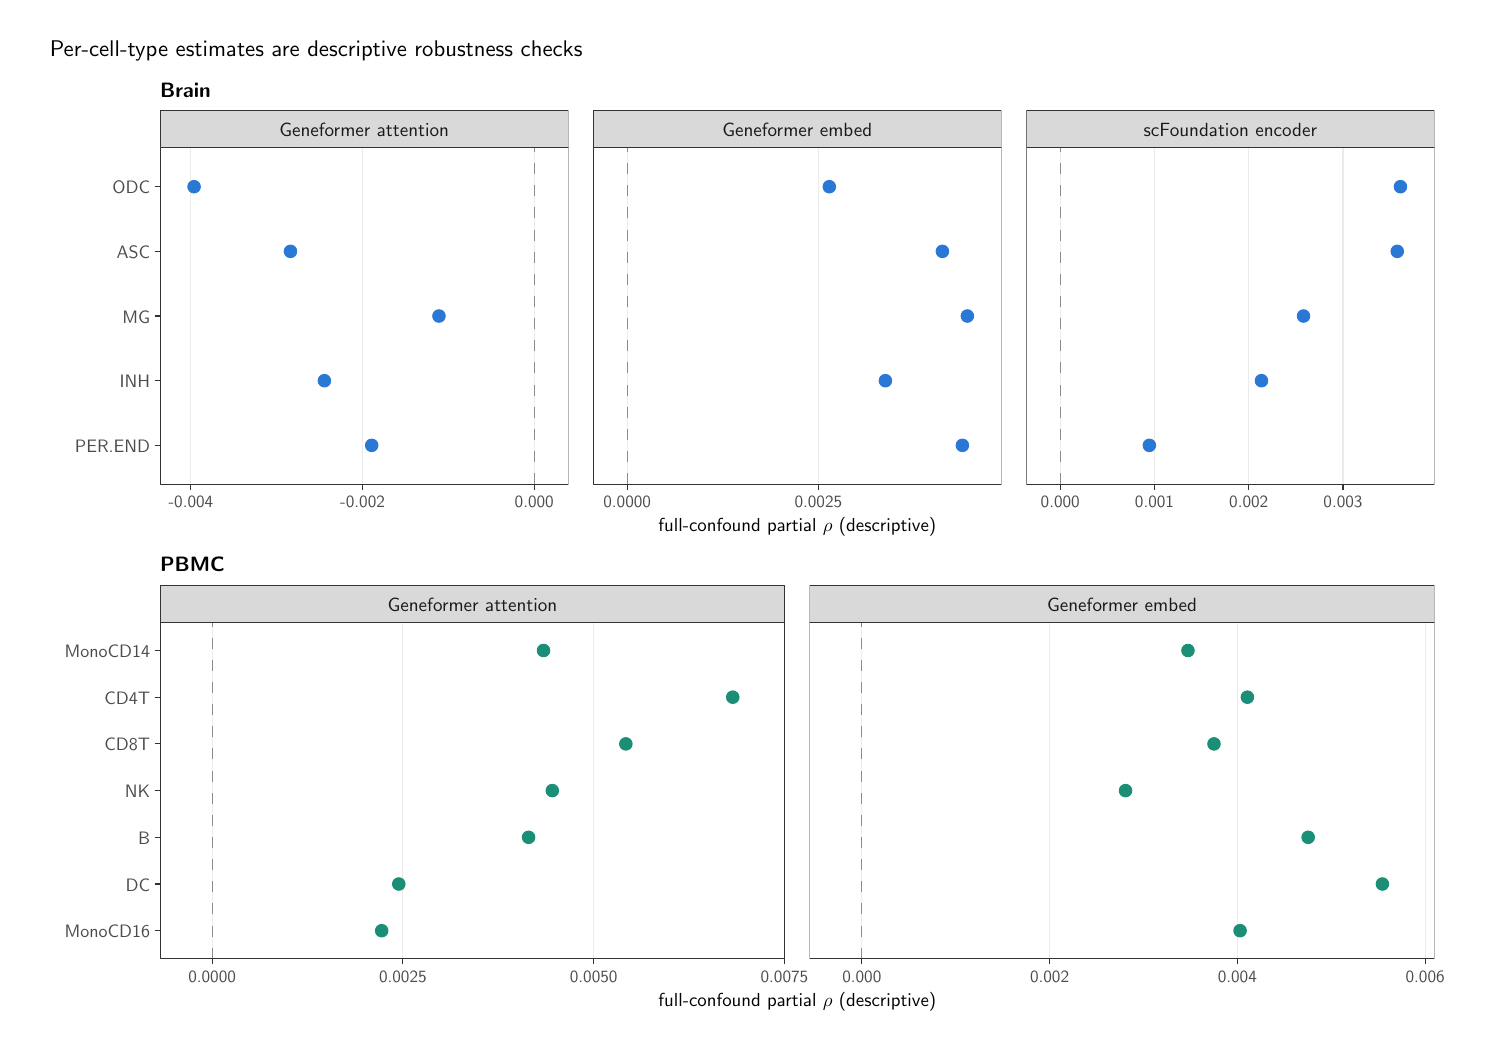
\begin{tikzpicture}[x=1pt,y=1pt]
\definecolor{fillColor}{RGB}{255,255,255}
\path[use as bounding box,fill=fillColor,fill opacity=0.00] (0,0) rectangle (520.34,361.35);
\begin{scope}
\path[clip] (  0.00,  0.00) rectangle (520.34,361.35);
\definecolor{drawColor}{RGB}{255,255,255}
\definecolor{fillColor}{RGB}{255,255,255}

\path[draw=drawColor,line width= 0.4pt,line join=round,line cap=round,fill=fillColor] ( -0.00,  0.00) rectangle (520.34,361.35);
\end{scope}
\begin{scope}
\path[clip] (  4.00,174.49) rectangle (514.34,345.97);
\definecolor{drawColor}{RGB}{255,255,255}
\definecolor{fillColor}{RGB}{255,255,255}

\path[draw=drawColor,line width= 0.4pt,line join=round,line cap=round,fill=fillColor] (  4.00,174.49) rectangle (514.34,345.97);
\end{scope}
\begin{scope}
\path[clip] (  4.00,  3.00) rectangle (514.34,174.49);
\definecolor{drawColor}{RGB}{255,255,255}
\definecolor{fillColor}{RGB}{255,255,255}

\path[draw=drawColor,line width= 0.4pt,line join=round,line cap=round,fill=fillColor] (  4.00,  3.00) rectangle (514.34,174.49);
\end{scope}
\begin{scope}
\path[clip] ( 47.84,196.40) rectangle (195.34,317.90);
\definecolor{fillColor}{RGB}{255,255,255}

\path[fill=fillColor] ( 47.84,196.40) rectangle (195.34,317.90);
\definecolor{drawColor}{gray}{0.92}

\path[draw=drawColor,line width= 0.4pt,line join=round] ( 58.99,196.40) --
	( 58.99,317.90);

\path[draw=drawColor,line width= 0.4pt,line join=round] (121.02,196.40) --
	(121.02,317.90);

\path[draw=drawColor,line width= 0.4pt,line join=round] (183.05,196.40) --
	(183.05,317.90);
\definecolor{drawColor}{gray}{0.55}

\path[draw=drawColor,line width= 0.4pt,dash pattern=on 4pt off 4pt ,line join=round] (183.05,196.40) -- (183.05,317.90);
\definecolor{drawColor}{RGB}{42,120,214}
\definecolor{fillColor}{RGB}{42,120,214}

\path[draw=drawColor,line width= 0.3pt,line join=round,line cap=round,fill=fillColor] ( 60.13,303.88) circle (  2.29);

\path[draw=drawColor,line width= 0.3pt,line join=round,line cap=round,fill=fillColor] ( 94.96,280.52) circle (  2.29);

\path[draw=drawColor,line width= 0.3pt,line join=round,line cap=round,fill=fillColor] (148.62,257.15) circle (  2.29);

\path[draw=drawColor,line width= 0.3pt,line join=round,line cap=round,fill=fillColor] (107.22,233.78) circle (  2.29);

\path[draw=drawColor,line width= 0.3pt,line join=round,line cap=round,fill=fillColor] (124.31,210.42) circle (  2.29);
\definecolor{drawColor}{gray}{0.20}

\path[draw=drawColor,line width= 0.4pt,line join=round,line cap=round] ( 47.84,196.40) rectangle (195.34,317.90);
\end{scope}
\begin{scope}
\path[clip] (204.34,196.40) rectangle (351.84,317.90);
\definecolor{fillColor}{RGB}{255,255,255}

\path[fill=fillColor] (204.34,196.40) rectangle (351.84,317.90);
\definecolor{drawColor}{gray}{0.92}

\path[draw=drawColor,line width= 0.4pt,line join=round] (216.63,196.40) --
	(216.63,317.90);

\path[draw=drawColor,line width= 0.4pt,line join=round] (285.72,196.40) --
	(285.72,317.90);
\definecolor{drawColor}{gray}{0.55}

\path[draw=drawColor,line width= 0.4pt,dash pattern=on 4pt off 4pt ,line join=round] (216.63,196.40) -- (216.63,317.90);
\definecolor{drawColor}{RGB}{42,120,214}
\definecolor{fillColor}{RGB}{42,120,214}

\path[draw=drawColor,line width= 0.3pt,line join=round,line cap=round,fill=fillColor] (289.67,303.88) circle (  2.29);

\path[draw=drawColor,line width= 0.3pt,line join=round,line cap=round,fill=fillColor] (330.54,280.52) circle (  2.29);

\path[draw=drawColor,line width= 0.3pt,line join=round,line cap=round,fill=fillColor] (339.55,257.15) circle (  2.29);

\path[draw=drawColor,line width= 0.3pt,line join=round,line cap=round,fill=fillColor] (309.93,233.78) circle (  2.29);

\path[draw=drawColor,line width= 0.3pt,line join=round,line cap=round,fill=fillColor] (337.76,210.42) circle (  2.29);
\definecolor{drawColor}{gray}{0.20}

\path[draw=drawColor,line width= 0.4pt,line join=round,line cap=round] (204.34,196.40) rectangle (351.84,317.90);
\end{scope}
\begin{scope}
\path[clip] (360.84,196.40) rectangle (508.34,317.90);
\definecolor{fillColor}{RGB}{255,255,255}

\path[fill=fillColor] (360.84,196.40) rectangle (508.34,317.90);
\definecolor{drawColor}{gray}{0.92}

\path[draw=drawColor,line width= 0.4pt,line join=round] (373.13,196.40) --
	(373.13,317.90);

\path[draw=drawColor,line width= 0.4pt,line join=round] (407.18,196.40) --
	(407.18,317.90);

\path[draw=drawColor,line width= 0.4pt,line join=round] (441.23,196.40) --
	(441.23,317.90);

\path[draw=drawColor,line width= 0.4pt,line join=round] (475.28,196.40) --
	(475.28,317.90);
\definecolor{drawColor}{gray}{0.55}

\path[draw=drawColor,line width= 0.4pt,dash pattern=on 4pt off 4pt ,line join=round] (373.13,196.40) -- (373.13,317.90);
\definecolor{drawColor}{RGB}{42,120,214}
\definecolor{fillColor}{RGB}{42,120,214}

\path[draw=drawColor,line width= 0.3pt,line join=round,line cap=round,fill=fillColor] (496.05,303.88) circle (  2.29);

\path[draw=drawColor,line width= 0.3pt,line join=round,line cap=round,fill=fillColor] (494.89,280.52) circle (  2.29);

\path[draw=drawColor,line width= 0.3pt,line join=round,line cap=round,fill=fillColor] (461.02,257.15) circle (  2.29);

\path[draw=drawColor,line width= 0.3pt,line join=round,line cap=round,fill=fillColor] (445.83,233.78) circle (  2.29);

\path[draw=drawColor,line width= 0.3pt,line join=round,line cap=round,fill=fillColor] (405.31,210.42) circle (  2.29);
\definecolor{drawColor}{gray}{0.20}

\path[draw=drawColor,line width= 0.4pt,line join=round,line cap=round] (360.84,196.40) rectangle (508.34,317.90);
\end{scope}
\begin{scope}
\path[clip] ( 47.84,317.90) rectangle (195.34,331.38);
\definecolor{drawColor}{gray}{0.20}
\definecolor{fillColor}{gray}{0.85}

\path[draw=drawColor,line width= 0.4pt,line join=round,line cap=round,fill=fillColor] ( 47.84,317.90) rectangle (195.34,331.38);
\definecolor{drawColor}{gray}{0.10}

\node[text=drawColor,anchor=base,inner sep=0pt, outer sep=0pt, scale=  0.69] at (121.59,321.95) {Geneformer attention};
\end{scope}
\begin{scope}
\path[clip] (204.34,317.90) rectangle (351.84,331.38);
\definecolor{drawColor}{gray}{0.20}
\definecolor{fillColor}{gray}{0.85}

\path[draw=drawColor,line width= 0.4pt,line join=round,line cap=round,fill=fillColor] (204.34,317.90) rectangle (351.84,331.38);
\definecolor{drawColor}{gray}{0.10}

\node[text=drawColor,anchor=base,inner sep=0pt, outer sep=0pt, scale=  0.69] at (278.09,321.95) {Geneformer embed};
\end{scope}
\begin{scope}
\path[clip] (360.84,317.90) rectangle (508.34,331.38);
\definecolor{drawColor}{gray}{0.20}
\definecolor{fillColor}{gray}{0.85}

\path[draw=drawColor,line width= 0.4pt,line join=round,line cap=round,fill=fillColor] (360.84,317.90) rectangle (508.34,331.38);
\definecolor{drawColor}{gray}{0.10}

\node[text=drawColor,anchor=base,inner sep=0pt, outer sep=0pt, scale=  0.69] at (434.59,321.95) {scFoundation encoder};
\end{scope}
\begin{scope}
\path[clip] (  0.00,  0.00) rectangle (520.34,361.35);
\definecolor{drawColor}{gray}{0.20}

\path[draw=drawColor,line width= 0.4pt,line join=round] ( 58.99,194.40) --
	( 58.99,196.40);

\path[draw=drawColor,line width= 0.4pt,line join=round] (121.02,194.40) --
	(121.02,196.40);

\path[draw=drawColor,line width= 0.4pt,line join=round] (183.05,194.40) --
	(183.05,196.40);
\end{scope}
\begin{scope}
\path[clip] (  0.00,  0.00) rectangle (520.34,361.35);
\definecolor{drawColor}{gray}{0.30}

\node[text=drawColor,anchor=base,inner sep=0pt, outer sep=0pt, scale=  0.62] at ( 58.99,187.97) {-0.004};

\node[text=drawColor,anchor=base,inner sep=0pt, outer sep=0pt, scale=  0.62] at (121.02,187.97) {-0.002};

\node[text=drawColor,anchor=base,inner sep=0pt, outer sep=0pt, scale=  0.62] at (183.05,187.97) {0.000};
\end{scope}
\begin{scope}
\path[clip] (  0.00,  0.00) rectangle (520.34,361.35);
\definecolor{drawColor}{gray}{0.20}

\path[draw=drawColor,line width= 0.4pt,line join=round] (216.63,194.40) --
	(216.63,196.40);

\path[draw=drawColor,line width= 0.4pt,line join=round] (285.72,194.40) --
	(285.72,196.40);
\end{scope}
\begin{scope}
\path[clip] (  0.00,  0.00) rectangle (520.34,361.35);
\definecolor{drawColor}{gray}{0.30}

\node[text=drawColor,anchor=base,inner sep=0pt, outer sep=0pt, scale=  0.62] at (216.63,187.97) {0.0000};

\node[text=drawColor,anchor=base,inner sep=0pt, outer sep=0pt, scale=  0.62] at (285.72,187.97) {0.0025};
\end{scope}
\begin{scope}
\path[clip] (  0.00,  0.00) rectangle (520.34,361.35);
\definecolor{drawColor}{gray}{0.20}

\path[draw=drawColor,line width= 0.4pt,line join=round] (373.13,194.40) --
	(373.13,196.40);

\path[draw=drawColor,line width= 0.4pt,line join=round] (407.18,194.40) --
	(407.18,196.40);

\path[draw=drawColor,line width= 0.4pt,line join=round] (441.23,194.40) --
	(441.23,196.40);

\path[draw=drawColor,line width= 0.4pt,line join=round] (475.28,194.40) --
	(475.28,196.40);
\end{scope}
\begin{scope}
\path[clip] (  0.00,  0.00) rectangle (520.34,361.35);
\definecolor{drawColor}{gray}{0.30}

\node[text=drawColor,anchor=base,inner sep=0pt, outer sep=0pt, scale=  0.62] at (373.13,187.97) {0.000};

\node[text=drawColor,anchor=base,inner sep=0pt, outer sep=0pt, scale=  0.62] at (407.18,187.97) {0.001};

\node[text=drawColor,anchor=base,inner sep=0pt, outer sep=0pt, scale=  0.62] at (441.23,187.97) {0.002};

\node[text=drawColor,anchor=base,inner sep=0pt, outer sep=0pt, scale=  0.62] at (475.28,187.97) {0.003};
\end{scope}
\begin{scope}
\path[clip] (  0.00,  0.00) rectangle (520.34,361.35);
\definecolor{drawColor}{gray}{0.30}

\node[text=drawColor,anchor=base east,inner sep=0pt, outer sep=0pt, scale=  0.65] at ( 44.24,207.86) {PER.END};

\node[text=drawColor,anchor=base east,inner sep=0pt, outer sep=0pt, scale=  0.65] at ( 44.24,231.23) {INH};

\node[text=drawColor,anchor=base east,inner sep=0pt, outer sep=0pt, scale=  0.65] at ( 44.24,254.60) {MG};

\node[text=drawColor,anchor=base east,inner sep=0pt, outer sep=0pt, scale=  0.65] at ( 44.24,277.96) {ASC};

\node[text=drawColor,anchor=base east,inner sep=0pt, outer sep=0pt, scale=  0.65] at ( 44.24,301.33) {ODC};
\end{scope}
\begin{scope}
\path[clip] (  0.00,  0.00) rectangle (520.34,361.35);
\definecolor{drawColor}{gray}{0.20}

\path[draw=drawColor,line width= 0.4pt,line join=round] ( 45.84,210.42) --
	( 47.84,210.42);

\path[draw=drawColor,line width= 0.4pt,line join=round] ( 45.84,233.78) --
	( 47.84,233.78);

\path[draw=drawColor,line width= 0.4pt,line join=round] ( 45.84,257.15) --
	( 47.84,257.15);

\path[draw=drawColor,line width= 0.4pt,line join=round] ( 45.84,280.52) --
	( 47.84,280.52);

\path[draw=drawColor,line width= 0.4pt,line join=round] ( 45.84,303.88) --
	( 47.84,303.88);
\end{scope}
\begin{scope}
\path[clip] (  0.00,  0.00) rectangle (520.34,361.35);
\definecolor{drawColor}{RGB}{0,0,0}

\node[text=drawColor,anchor=base,inner sep=0pt, outer sep=0pt, scale=  0.68] at (278.09,179.15) {full-confound partial $\rho$ (descriptive)};
\end{scope}
\begin{scope}
\path[clip] (  0.00,  0.00) rectangle (520.34,361.35);
\definecolor{drawColor}{RGB}{0,0,0}

\node[text=drawColor,anchor=base west,inner sep=0pt, outer sep=0pt, scale=  0.75] at ( 47.84,336.19) {\bfseries Brain};
\end{scope}
\begin{scope}
\path[clip] ( 47.84, 24.91) rectangle (273.59,146.42);
\definecolor{fillColor}{RGB}{255,255,255}

\path[fill=fillColor] ( 47.84, 24.91) rectangle (273.59,146.42);
\definecolor{drawColor}{gray}{0.92}

\path[draw=drawColor,line width= 0.4pt,line join=round] ( 66.65, 24.91) --
	( 66.65,146.42);

\path[draw=drawColor,line width= 0.4pt,line join=round] (135.59, 24.91) --
	(135.59,146.42);

\path[draw=drawColor,line width= 0.4pt,line join=round] (204.52, 24.91) --
	(204.52,146.42);

\path[draw=drawColor,line width= 0.4pt,line join=round] (273.45, 24.91) --
	(273.45,146.42);
\definecolor{drawColor}{gray}{0.55}

\path[draw=drawColor,line width= 0.4pt,dash pattern=on 4pt off 4pt ,line join=round] ( 66.65, 24.91) -- ( 66.65,146.42);
\definecolor{drawColor}{RGB}{27,143,117}
\definecolor{fillColor}{RGB}{27,143,117}

\path[draw=drawColor,line width= 0.3pt,line join=round,line cap=round,fill=fillColor] (186.40,136.29) circle (  2.29);

\path[draw=drawColor,line width= 0.3pt,line join=round,line cap=round,fill=fillColor] (254.78,119.42) circle (  2.29);

\path[draw=drawColor,line width= 0.3pt,line join=round,line cap=round,fill=fillColor] (216.15,102.54) circle (  2.29);

\path[draw=drawColor,line width= 0.3pt,line join=round,line cap=round,fill=fillColor] (189.57, 85.66) circle (  2.29);

\path[draw=drawColor,line width= 0.3pt,line join=round,line cap=round,fill=fillColor] (181.00, 68.79) circle (  2.29);

\path[draw=drawColor,line width= 0.3pt,line join=round,line cap=round,fill=fillColor] (134.10, 51.91) circle (  2.29);

\path[draw=drawColor,line width= 0.3pt,line join=round,line cap=round,fill=fillColor] (127.92, 35.04) circle (  2.29);
\definecolor{drawColor}{gray}{0.20}

\path[draw=drawColor,line width= 0.4pt,line join=round,line cap=round] ( 47.84, 24.91) rectangle (273.59,146.42);
\end{scope}
\begin{scope}
\path[clip] (282.59, 24.91) rectangle (508.34,146.42);
\definecolor{fillColor}{RGB}{255,255,255}

\path[fill=fillColor] (282.59, 24.91) rectangle (508.34,146.42);
\definecolor{drawColor}{gray}{0.92}

\path[draw=drawColor,line width= 0.4pt,line join=round] (301.41, 24.91) --
	(301.41,146.42);

\path[draw=drawColor,line width= 0.4pt,line join=round] (369.26, 24.91) --
	(369.26,146.42);

\path[draw=drawColor,line width= 0.4pt,line join=round] (437.11, 24.91) --
	(437.11,146.42);

\path[draw=drawColor,line width= 0.4pt,line join=round] (504.97, 24.91) --
	(504.97,146.42);
\definecolor{drawColor}{gray}{0.55}

\path[draw=drawColor,line width= 0.4pt,dash pattern=on 4pt off 4pt ,line join=round] (301.41, 24.91) -- (301.41,146.42);
\definecolor{drawColor}{RGB}{27,143,117}
\definecolor{fillColor}{RGB}{27,143,117}

\path[draw=drawColor,line width= 0.3pt,line join=round,line cap=round,fill=fillColor] (419.27,136.29) circle (  2.29);

\path[draw=drawColor,line width= 0.3pt,line join=round,line cap=round,fill=fillColor] (440.74,119.42) circle (  2.29);

\path[draw=drawColor,line width= 0.3pt,line join=round,line cap=round,fill=fillColor] (428.67,102.54) circle (  2.29);

\path[draw=drawColor,line width= 0.3pt,line join=round,line cap=round,fill=fillColor] (396.71, 85.66) circle (  2.29);

\path[draw=drawColor,line width= 0.3pt,line join=round,line cap=round,fill=fillColor] (462.70, 68.79) circle (  2.29);

\path[draw=drawColor,line width= 0.3pt,line join=round,line cap=round,fill=fillColor] (489.53, 51.91) circle (  2.29);

\path[draw=drawColor,line width= 0.3pt,line join=round,line cap=round,fill=fillColor] (438.10, 35.04) circle (  2.29);
\definecolor{drawColor}{gray}{0.20}

\path[draw=drawColor,line width= 0.4pt,line join=round,line cap=round] (282.59, 24.91) rectangle (508.34,146.42);
\end{scope}
\begin{scope}
\path[clip] ( 47.84,146.42) rectangle (273.59,159.89);
\definecolor{drawColor}{gray}{0.20}
\definecolor{fillColor}{gray}{0.85}

\path[draw=drawColor,line width= 0.4pt,line join=round,line cap=round,fill=fillColor] ( 47.84,146.42) rectangle (273.59,159.89);
\definecolor{drawColor}{gray}{0.10}

\node[text=drawColor,anchor=base,inner sep=0pt, outer sep=0pt, scale=  0.69] at (160.72,150.46) {Geneformer attention};
\end{scope}
\begin{scope}
\path[clip] (282.59,146.42) rectangle (508.34,159.89);
\definecolor{drawColor}{gray}{0.20}
\definecolor{fillColor}{gray}{0.85}

\path[draw=drawColor,line width= 0.4pt,line join=round,line cap=round,fill=fillColor] (282.59,146.42) rectangle (508.34,159.89);
\definecolor{drawColor}{gray}{0.10}

\node[text=drawColor,anchor=base,inner sep=0pt, outer sep=0pt, scale=  0.69] at (395.47,150.46) {Geneformer embed};
\end{scope}
\begin{scope}
\path[clip] (  0.00,  0.00) rectangle (520.34,361.35);
\definecolor{drawColor}{gray}{0.20}

\path[draw=drawColor,line width= 0.4pt,line join=round] ( 66.65, 22.91) --
	( 66.65, 24.91);

\path[draw=drawColor,line width= 0.4pt,line join=round] (135.59, 22.91) --
	(135.59, 24.91);

\path[draw=drawColor,line width= 0.4pt,line join=round] (204.52, 22.91) --
	(204.52, 24.91);

\path[draw=drawColor,line width= 0.4pt,line join=round] (273.45, 22.91) --
	(273.45, 24.91);
\end{scope}
\begin{scope}
\path[clip] (  0.00,  0.00) rectangle (520.34,361.35);
\definecolor{drawColor}{gray}{0.30}

\node[text=drawColor,anchor=base,inner sep=0pt, outer sep=0pt, scale=  0.62] at ( 66.65, 16.49) {0.0000};

\node[text=drawColor,anchor=base,inner sep=0pt, outer sep=0pt, scale=  0.62] at (135.59, 16.49) {0.0025};

\node[text=drawColor,anchor=base,inner sep=0pt, outer sep=0pt, scale=  0.62] at (204.52, 16.49) {0.0050};

\node[text=drawColor,anchor=base,inner sep=0pt, outer sep=0pt, scale=  0.62] at (273.45, 16.49) {0.0075};
\end{scope}
\begin{scope}
\path[clip] (  0.00,  0.00) rectangle (520.34,361.35);
\definecolor{drawColor}{gray}{0.20}

\path[draw=drawColor,line width= 0.4pt,line join=round] (301.41, 22.91) --
	(301.41, 24.91);

\path[draw=drawColor,line width= 0.4pt,line join=round] (369.26, 22.91) --
	(369.26, 24.91);

\path[draw=drawColor,line width= 0.4pt,line join=round] (437.11, 22.91) --
	(437.11, 24.91);

\path[draw=drawColor,line width= 0.4pt,line join=round] (504.97, 22.91) --
	(504.97, 24.91);
\end{scope}
\begin{scope}
\path[clip] (  0.00,  0.00) rectangle (520.34,361.35);
\definecolor{drawColor}{gray}{0.30}

\node[text=drawColor,anchor=base,inner sep=0pt, outer sep=0pt, scale=  0.62] at (301.41, 16.49) {0.000};

\node[text=drawColor,anchor=base,inner sep=0pt, outer sep=0pt, scale=  0.62] at (369.26, 16.49) {0.002};

\node[text=drawColor,anchor=base,inner sep=0pt, outer sep=0pt, scale=  0.62] at (437.11, 16.49) {0.004};

\node[text=drawColor,anchor=base,inner sep=0pt, outer sep=0pt, scale=  0.62] at (504.97, 16.49) {0.006};
\end{scope}
\begin{scope}
\path[clip] (  0.00,  0.00) rectangle (520.34,361.35);
\definecolor{drawColor}{gray}{0.30}

\node[text=drawColor,anchor=base east,inner sep=0pt, outer sep=0pt, scale=  0.65] at ( 44.24, 32.48) {MonoCD16};

\node[text=drawColor,anchor=base east,inner sep=0pt, outer sep=0pt, scale=  0.65] at ( 44.24, 49.36) {DC};

\node[text=drawColor,anchor=base east,inner sep=0pt, outer sep=0pt, scale=  0.65] at ( 44.24, 66.23) {B};

\node[text=drawColor,anchor=base east,inner sep=0pt, outer sep=0pt, scale=  0.65] at ( 44.24, 83.11) {NK};

\node[text=drawColor,anchor=base east,inner sep=0pt, outer sep=0pt, scale=  0.65] at ( 44.24, 99.99) {CD8T};

\node[text=drawColor,anchor=base east,inner sep=0pt, outer sep=0pt, scale=  0.65] at ( 44.24,116.86) {CD4T};

\node[text=drawColor,anchor=base east,inner sep=0pt, outer sep=0pt, scale=  0.65] at ( 44.24,133.74) {MonoCD14};
\end{scope}
\begin{scope}
\path[clip] (  0.00,  0.00) rectangle (520.34,361.35);
\definecolor{drawColor}{gray}{0.20}

\path[draw=drawColor,line width= 0.4pt,line join=round] ( 45.84, 35.04) --
	( 47.84, 35.04);

\path[draw=drawColor,line width= 0.4pt,line join=round] ( 45.84, 51.91) --
	( 47.84, 51.91);

\path[draw=drawColor,line width= 0.4pt,line join=round] ( 45.84, 68.79) --
	( 47.84, 68.79);

\path[draw=drawColor,line width= 0.4pt,line join=round] ( 45.84, 85.66) --
	( 47.84, 85.66);

\path[draw=drawColor,line width= 0.4pt,line join=round] ( 45.84,102.54) --
	( 47.84,102.54);

\path[draw=drawColor,line width= 0.4pt,line join=round] ( 45.84,119.42) --
	( 47.84,119.42);

\path[draw=drawColor,line width= 0.4pt,line join=round] ( 45.84,136.29) --
	( 47.84,136.29);
\end{scope}
\begin{scope}
\path[clip] (  0.00,  0.00) rectangle (520.34,361.35);
\definecolor{drawColor}{RGB}{0,0,0}

\node[text=drawColor,anchor=base,inner sep=0pt, outer sep=0pt, scale=  0.68] at (278.09,  7.66) {full-confound partial $\rho$ (descriptive)};
\end{scope}
\begin{scope}
\path[clip] (  0.00,  0.00) rectangle (520.34,361.35);
\definecolor{drawColor}{RGB}{0,0,0}

\node[text=drawColor,anchor=base west,inner sep=0pt, outer sep=0pt, scale=  0.75] at ( 47.84,164.71) {\bfseries PBMC};
\end{scope}
\begin{scope}
\path[clip] (  0.00,  0.00) rectangle (520.34,361.35);
\definecolor{drawColor}{RGB}{0,0,0}

\node[text=drawColor,anchor=base west,inner sep=0pt, outer sep=0pt, scale=  0.82] at (  8.00,350.97) {Per-cell-type estimates are descriptive robustness checks};
\end{scope}
\end{tikzpicture}
}
\caption{Per-cell-type full-confound estimates. These observed effects are descriptive exploratory
robustness checks without randomization $p$-values or multiplicity claims.}\label{fig:pertype}
\end{figure}

\begin{figure}[t]\centering
\resizebox{\textwidth}{!}{% Created by tikzDevice version 0.12.6 on 2026-08-01 04:31:26
% !TEX encoding = UTF-8 Unicode
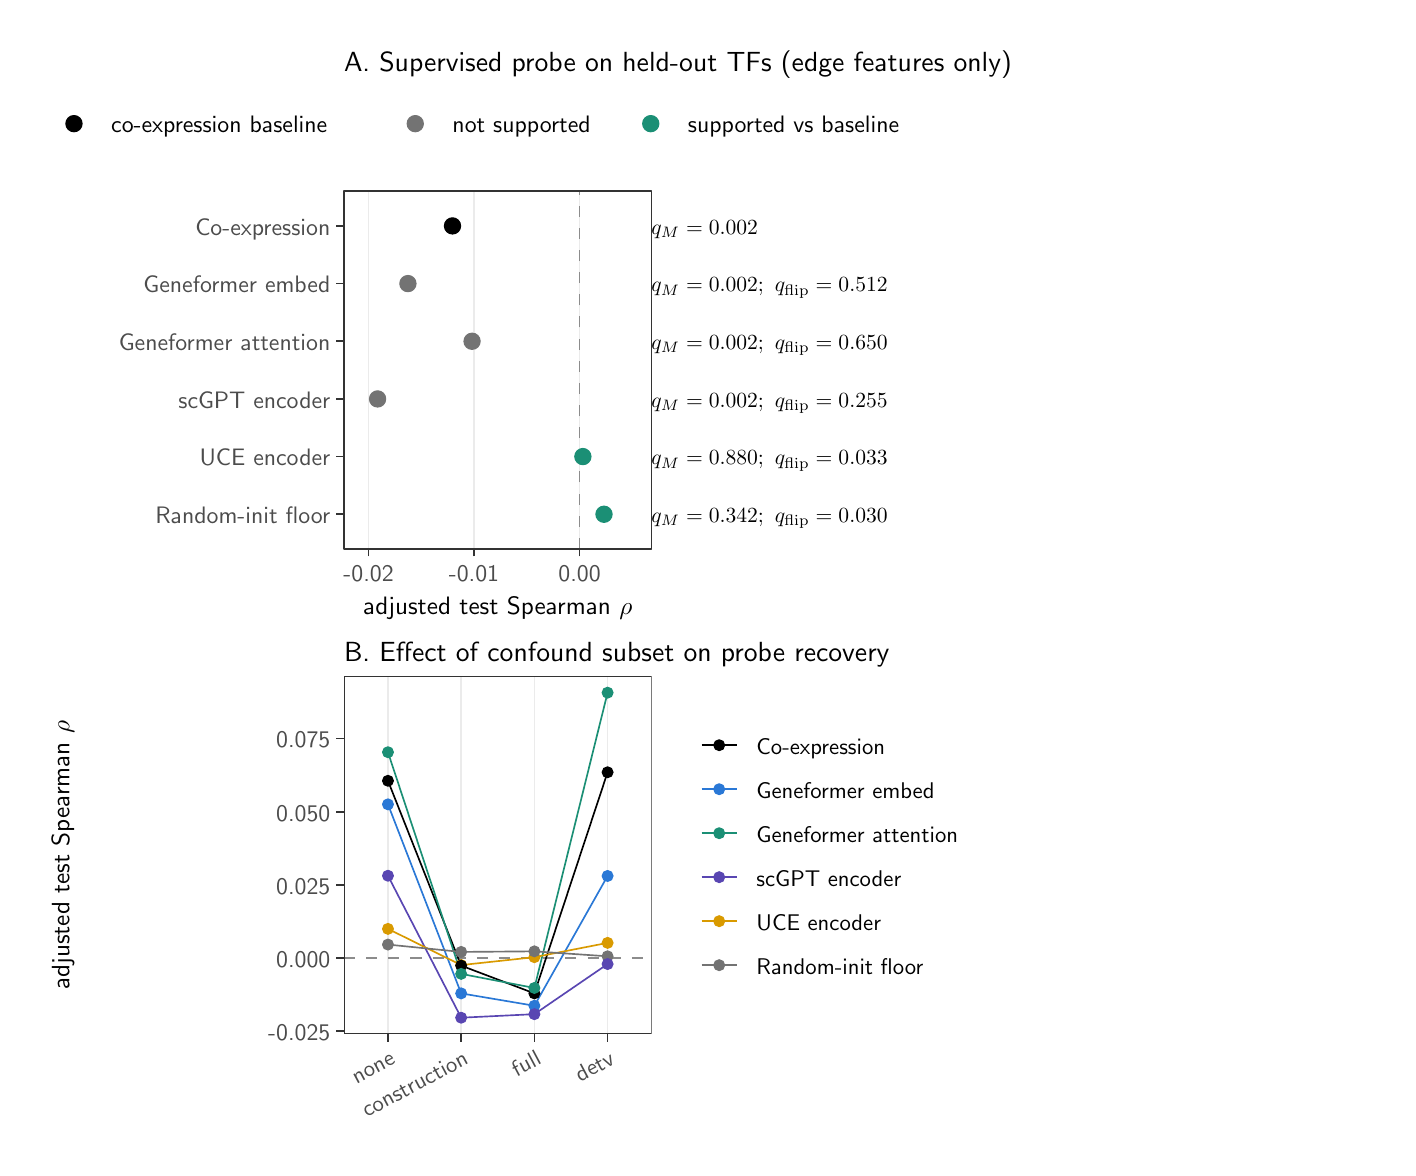
\begin{tikzpicture}[x=1pt,y=1pt]
\definecolor{fillColor}{RGB}{255,255,255}
\path[use as bounding box,fill=fillColor,fill opacity=0.00] (0,0) rectangle (491.44,404.71);
\begin{scope}
\path[clip] (  0.00,  0.00) rectangle (491.44,404.71);
\definecolor{drawColor}{RGB}{255,255,255}
\definecolor{fillColor}{RGB}{255,255,255}

\path[draw=drawColor,line width= 0.6pt,line join=round,line cap=round,fill=fillColor] (  0.00,  0.00) rectangle (491.44,404.71);
\end{scope}
\begin{scope}
\path[clip] (  4.00,187.52) rectangle (485.44,400.71);
\definecolor{drawColor}{RGB}{255,255,255}
\definecolor{fillColor}{RGB}{255,255,255}

\path[draw=drawColor,line width= 0.6pt,line join=round,line cap=round,fill=fillColor] (  4.00,187.52) rectangle (485.44,400.71);
\end{scope}
\begin{scope}
\path[clip] (  4.00,  3.00) rectangle (485.44,187.52);
\definecolor{drawColor}{RGB}{255,255,255}
\definecolor{fillColor}{RGB}{255,255,255}

\path[draw=drawColor,line width= 0.6pt,line join=round,line cap=round,fill=fillColor] (  4.00,  3.00) rectangle (485.44,187.52);
\end{scope}
\begin{scope}
\path[clip] (  0.00,  0.00) rectangle (491.44,404.71);
\definecolor{fillColor}{RGB}{255,255,255}

\path[fill=fillColor] (114.31,216.37) rectangle (225.43,345.57);
\definecolor{drawColor}{gray}{0.92}

\path[draw=drawColor,line width= 0.6pt,line join=round] (123.18,216.37) --
	(123.18,345.57);

\path[draw=drawColor,line width= 0.6pt,line join=round] (161.29,216.37) --
	(161.29,345.57);

\path[draw=drawColor,line width= 0.6pt,line join=round] (199.41,216.37) --
	(199.41,345.57);
\definecolor{drawColor}{gray}{0.55}

\path[draw=drawColor,line width= 0.6pt,dash pattern=on 4pt off 4pt ,line join=round] (199.41,216.37) -- (199.41,345.57);
\definecolor{drawColor}{RGB}{27,143,117}
\definecolor{fillColor}{RGB}{27,143,117}

\path[draw=drawColor,line width= 0.4pt,line join=round,line cap=round,fill=fillColor] (200.62,249.72) circle (  2.93);
\definecolor{drawColor}{RGB}{0,0,0}
\definecolor{fillColor}{RGB}{0,0,0}

\path[draw=drawColor,line width= 0.4pt,line join=round,line cap=round,fill=fillColor] (153.51,333.07) circle (  2.93);
\definecolor{drawColor}{gray}{0.45}
\definecolor{fillColor}{gray}{0.45}

\path[draw=drawColor,line width= 0.4pt,line join=round,line cap=round,fill=fillColor] (160.58,291.39) circle (  2.93);

\path[draw=drawColor,line width= 0.4pt,line join=round,line cap=round,fill=fillColor] (137.40,312.23) circle (  2.93);
\definecolor{drawColor}{RGB}{27,143,117}
\definecolor{fillColor}{RGB}{27,143,117}

\path[draw=drawColor,line width= 0.4pt,line join=round,line cap=round,fill=fillColor] (208.25,228.88) circle (  2.93);
\definecolor{drawColor}{gray}{0.45}
\definecolor{fillColor}{gray}{0.45}

\path[draw=drawColor,line width= 0.4pt,line join=round,line cap=round,fill=fillColor] (126.44,270.55) circle (  2.93);
\definecolor{drawColor}{RGB}{0,0,0}

\node[text=drawColor,anchor=base west,inner sep=0pt, outer sep=0pt, scale=  0.78] at (225.33,246.69) {$q_M=0.880;\ q_{\mathrm{flip}}=0.033$};

\node[text=drawColor,anchor=base west,inner sep=0pt, outer sep=0pt, scale=  0.78] at (225.33,330.04) {$q_M=0.002$};

\node[text=drawColor,anchor=base west,inner sep=0pt, outer sep=0pt, scale=  0.78] at (225.33,288.37) {$q_M=0.002;\ q_{\mathrm{flip}}=0.650$};

\node[text=drawColor,anchor=base west,inner sep=0pt, outer sep=0pt, scale=  0.78] at (225.33,309.21) {$q_M=0.002;\ q_{\mathrm{flip}}=0.512$};

\node[text=drawColor,anchor=base west,inner sep=0pt, outer sep=0pt, scale=  0.78] at (225.33,225.85) {$q_M=0.342;\ q_{\mathrm{flip}}=0.030$};

\node[text=drawColor,anchor=base west,inner sep=0pt, outer sep=0pt, scale=  0.78] at (225.33,267.53) {$q_M=0.002;\ q_{\mathrm{flip}}=0.255$};
\definecolor{drawColor}{gray}{0.20}

\path[draw=drawColor,line width= 0.6pt,line join=round,line cap=round] (114.31,216.37) rectangle (225.43,345.57);
\end{scope}
\begin{scope}
\path[clip] (  0.00,  0.00) rectangle (491.44,404.71);
\definecolor{drawColor}{gray}{0.30}

\node[text=drawColor,anchor=base east,inner sep=0pt, outer sep=0pt, scale=  0.86] at (109.36,225.51) {Random-init floor};

\node[text=drawColor,anchor=base east,inner sep=0pt, outer sep=0pt, scale=  0.86] at (109.36,246.35) {UCE encoder};

\node[text=drawColor,anchor=base east,inner sep=0pt, outer sep=0pt, scale=  0.86] at (109.36,267.19) {scGPT encoder};

\node[text=drawColor,anchor=base east,inner sep=0pt, outer sep=0pt, scale=  0.86] at (109.36,288.02) {Geneformer attention};

\node[text=drawColor,anchor=base east,inner sep=0pt, outer sep=0pt, scale=  0.86] at (109.36,308.86) {Geneformer embed};

\node[text=drawColor,anchor=base east,inner sep=0pt, outer sep=0pt, scale=  0.86] at (109.36,329.70) {Co-expression};
\end{scope}
\begin{scope}
\path[clip] (  0.00,  0.00) rectangle (491.44,404.71);
\definecolor{drawColor}{gray}{0.20}

\path[draw=drawColor,line width= 0.6pt,line join=round] (111.56,228.88) --
	(114.31,228.88);

\path[draw=drawColor,line width= 0.6pt,line join=round] (111.56,249.72) --
	(114.31,249.72);

\path[draw=drawColor,line width= 0.6pt,line join=round] (111.56,270.55) --
	(114.31,270.55);

\path[draw=drawColor,line width= 0.6pt,line join=round] (111.56,291.39) --
	(114.31,291.39);

\path[draw=drawColor,line width= 0.6pt,line join=round] (111.56,312.23) --
	(114.31,312.23);

\path[draw=drawColor,line width= 0.6pt,line join=round] (111.56,333.07) --
	(114.31,333.07);
\end{scope}
\begin{scope}
\path[clip] (  0.00,  0.00) rectangle (491.44,404.71);
\definecolor{drawColor}{gray}{0.20}

\path[draw=drawColor,line width= 0.6pt,line join=round] (123.18,213.62) --
	(123.18,216.37);

\path[draw=drawColor,line width= 0.6pt,line join=round] (161.29,213.62) --
	(161.29,216.37);

\path[draw=drawColor,line width= 0.6pt,line join=round] (199.41,213.62) --
	(199.41,216.37);
\end{scope}
\begin{scope}
\path[clip] (  0.00,  0.00) rectangle (491.44,404.71);
\definecolor{drawColor}{gray}{0.30}

\node[text=drawColor,anchor=base,inner sep=0pt, outer sep=0pt, scale=  0.86] at (123.18,204.69) {-0.02};

\node[text=drawColor,anchor=base,inner sep=0pt, outer sep=0pt, scale=  0.86] at (161.29,204.69) {-0.01};

\node[text=drawColor,anchor=base,inner sep=0pt, outer sep=0pt, scale=  0.86] at (199.41,204.69) {0.00};
\end{scope}
\begin{scope}
\path[clip] (  0.00,  0.00) rectangle (491.44,404.71);
\definecolor{drawColor}{RGB}{0,0,0}

\node[text=drawColor,anchor=base,inner sep=0pt, outer sep=0pt, scale=  0.91] at (169.87,192.74) {adjusted test Spearman $\rho$};
\end{scope}
\begin{scope}
\path[clip] (  0.00,  0.00) rectangle (491.44,404.71);
\definecolor{fillColor}{RGB}{255,255,255}

\path[fill=fillColor] (  3.28,356.57) rectangle (336.46,383.47);
\end{scope}
\begin{scope}
\path[clip] (  0.00,  0.00) rectangle (491.44,404.71);
\definecolor{fillColor}{RGB}{255,255,255}

\path[fill=fillColor] (  8.78,362.07) rectangle ( 24.68,377.97);
\definecolor{drawColor}{RGB}{0,0,0}
\definecolor{fillColor}{RGB}{0,0,0}

\path[draw=drawColor,line width= 0.4pt,line join=round,line cap=round,fill=fillColor] ( 16.73,370.02) circle (  2.93);
\end{scope}
\begin{scope}
\path[clip] (  0.00,  0.00) rectangle (491.44,404.71);
\definecolor{fillColor}{RGB}{255,255,255}

\path[fill=fillColor] (132.10,362.07) rectangle (148.00,377.97);
\definecolor{drawColor}{gray}{0.45}
\definecolor{fillColor}{gray}{0.45}

\path[draw=drawColor,line width= 0.4pt,line join=round,line cap=round,fill=fillColor] (140.05,370.02) circle (  2.93);
\end{scope}
\begin{scope}
\path[clip] (  0.00,  0.00) rectangle (491.44,404.71);
\definecolor{fillColor}{RGB}{255,255,255}

\path[fill=fillColor] (217.20,362.07) rectangle (233.10,377.97);
\definecolor{drawColor}{RGB}{27,143,117}
\definecolor{fillColor}{RGB}{27,143,117}

\path[draw=drawColor,line width= 0.4pt,line join=round,line cap=round,fill=fillColor] (225.15,370.02) circle (  2.93);
\end{scope}
\begin{scope}
\path[clip] (  0.00,  0.00) rectangle (491.44,404.71);
\definecolor{drawColor}{RGB}{0,0,0}

\node[text=drawColor,anchor=base west,inner sep=0pt, outer sep=0pt, scale=  0.86] at ( 30.18,366.66) {co-expression baseline};
\end{scope}
\begin{scope}
\path[clip] (  0.00,  0.00) rectangle (491.44,404.71);
\definecolor{drawColor}{RGB}{0,0,0}

\node[text=drawColor,anchor=base west,inner sep=0pt, outer sep=0pt, scale=  0.86] at (153.50,366.66) {not supported};
\end{scope}
\begin{scope}
\path[clip] (  0.00,  0.00) rectangle (491.44,404.71);
\definecolor{drawColor}{RGB}{0,0,0}

\node[text=drawColor,anchor=base west,inner sep=0pt, outer sep=0pt, scale=  0.86] at (238.60,366.66) {supported vs baseline};
\end{scope}
\begin{scope}
\path[clip] (  0.00,  0.00) rectangle (491.44,404.71);
\definecolor{drawColor}{RGB}{0,0,0}

\node[text=drawColor,anchor=base west,inner sep=0pt, outer sep=0pt, scale=  1.00] at (114.31,388.91) {A. Supervised probe on held-out TFs (edge features only)};
\end{scope}
\begin{scope}
\path[clip] (114.31, 41.08) rectangle (225.43,170.29);
\definecolor{fillColor}{RGB}{255,255,255}

\path[fill=fillColor] (114.31, 41.08) rectangle (225.43,170.29);
\definecolor{drawColor}{gray}{0.92}

\path[draw=drawColor,line width= 0.6pt,line join=round] (130.19, 41.08) --
	(130.19,170.29);

\path[draw=drawColor,line width= 0.6pt,line join=round] (156.64, 41.08) --
	(156.64,170.29);

\path[draw=drawColor,line width= 0.6pt,line join=round] (183.10, 41.08) --
	(183.10,170.29);

\path[draw=drawColor,line width= 0.6pt,line join=round] (209.55, 41.08) --
	(209.55,170.29);
\definecolor{drawColor}{gray}{0.55}

\path[draw=drawColor,line width= 0.6pt,dash pattern=on 4pt off 4pt ,line join=round] (114.31, 68.49) -- (225.43, 68.49);
\definecolor{drawColor}{RGB}{0,0,0}

\path[draw=drawColor,line width= 0.6pt,line join=round] (130.19,132.57) --
	(156.64, 65.78) --
	(183.10, 55.75) --
	(209.55,135.65);
\definecolor{drawColor}{RGB}{42,120,214}

\path[draw=drawColor,line width= 0.6pt,line join=round] (130.19,124.06) --
	(156.64, 55.75) --
	(183.10, 51.28) --
	(209.55, 98.18);
\definecolor{drawColor}{RGB}{27,143,117}

\path[draw=drawColor,line width= 0.6pt,line join=round] (130.19,142.90) --
	(156.64, 62.80) --
	(183.10, 57.71) --
	(209.55,164.41);
\definecolor{drawColor}{RGB}{89,70,178}

\path[draw=drawColor,line width= 0.6pt,line join=round] (130.19, 98.26) --
	(156.64, 46.96) --
	(183.10, 48.24) --
	(209.55, 66.35);
\definecolor{drawColor}{RGB}{217,154,0}

\path[draw=drawColor,line width= 0.6pt,line join=round] (130.19, 79.06) --
	(156.64, 65.98) --
	(183.10, 68.83) --
	(209.55, 74.00);
\definecolor{drawColor}{gray}{0.45}

\path[draw=drawColor,line width= 0.6pt,line join=round] (130.19, 73.39) --
	(156.64, 70.73) --
	(183.10, 70.94) --
	(209.55, 69.15);
\definecolor{drawColor}{RGB}{217,154,0}
\definecolor{fillColor}{RGB}{217,154,0}

\path[draw=drawColor,line width= 0.4pt,line join=round,line cap=round,fill=fillColor] (156.64, 65.98) circle (  1.96);

\path[draw=drawColor,line width= 0.4pt,line join=round,line cap=round,fill=fillColor] (209.55, 74.00) circle (  1.96);

\path[draw=drawColor,line width= 0.4pt,line join=round,line cap=round,fill=fillColor] (183.10, 68.83) circle (  1.96);

\path[draw=drawColor,line width= 0.4pt,line join=round,line cap=round,fill=fillColor] (130.19, 79.06) circle (  1.96);
\definecolor{drawColor}{RGB}{0,0,0}
\definecolor{fillColor}{RGB}{0,0,0}

\path[draw=drawColor,line width= 0.4pt,line join=round,line cap=round,fill=fillColor] (156.64, 65.78) circle (  1.96);

\path[draw=drawColor,line width= 0.4pt,line join=round,line cap=round,fill=fillColor] (209.55,135.65) circle (  1.96);

\path[draw=drawColor,line width= 0.4pt,line join=round,line cap=round,fill=fillColor] (183.10, 55.75) circle (  1.96);

\path[draw=drawColor,line width= 0.4pt,line join=round,line cap=round,fill=fillColor] (130.19,132.57) circle (  1.96);
\definecolor{drawColor}{RGB}{27,143,117}
\definecolor{fillColor}{RGB}{27,143,117}

\path[draw=drawColor,line width= 0.4pt,line join=round,line cap=round,fill=fillColor] (156.64, 62.80) circle (  1.96);

\path[draw=drawColor,line width= 0.4pt,line join=round,line cap=round,fill=fillColor] (209.55,164.41) circle (  1.96);

\path[draw=drawColor,line width= 0.4pt,line join=round,line cap=round,fill=fillColor] (183.10, 57.71) circle (  1.96);

\path[draw=drawColor,line width= 0.4pt,line join=round,line cap=round,fill=fillColor] (130.19,142.90) circle (  1.96);
\definecolor{drawColor}{RGB}{42,120,214}
\definecolor{fillColor}{RGB}{42,120,214}

\path[draw=drawColor,line width= 0.4pt,line join=round,line cap=round,fill=fillColor] (156.64, 55.75) circle (  1.96);

\path[draw=drawColor,line width= 0.4pt,line join=round,line cap=round,fill=fillColor] (209.55, 98.18) circle (  1.96);

\path[draw=drawColor,line width= 0.4pt,line join=round,line cap=round,fill=fillColor] (183.10, 51.28) circle (  1.96);

\path[draw=drawColor,line width= 0.4pt,line join=round,line cap=round,fill=fillColor] (130.19,124.06) circle (  1.96);
\definecolor{drawColor}{gray}{0.45}
\definecolor{fillColor}{gray}{0.45}

\path[draw=drawColor,line width= 0.4pt,line join=round,line cap=round,fill=fillColor] (156.64, 70.73) circle (  1.96);

\path[draw=drawColor,line width= 0.4pt,line join=round,line cap=round,fill=fillColor] (209.55, 69.15) circle (  1.96);

\path[draw=drawColor,line width= 0.4pt,line join=round,line cap=round,fill=fillColor] (183.10, 70.94) circle (  1.96);

\path[draw=drawColor,line width= 0.4pt,line join=round,line cap=round,fill=fillColor] (130.19, 73.39) circle (  1.96);
\definecolor{drawColor}{RGB}{89,70,178}
\definecolor{fillColor}{RGB}{89,70,178}

\path[draw=drawColor,line width= 0.4pt,line join=round,line cap=round,fill=fillColor] (156.64, 46.96) circle (  1.96);

\path[draw=drawColor,line width= 0.4pt,line join=round,line cap=round,fill=fillColor] (209.55, 66.35) circle (  1.96);

\path[draw=drawColor,line width= 0.4pt,line join=round,line cap=round,fill=fillColor] (183.10, 48.24) circle (  1.96);

\path[draw=drawColor,line width= 0.4pt,line join=round,line cap=round,fill=fillColor] (130.19, 98.26) circle (  1.96);
\definecolor{drawColor}{gray}{0.20}

\path[draw=drawColor,line width= 0.6pt,line join=round,line cap=round] (114.31, 41.08) rectangle (225.43,170.29);
\end{scope}
\begin{scope}
\path[clip] (  0.00,  0.00) rectangle (491.44,404.71);
\definecolor{drawColor}{gray}{0.30}

\node[text=drawColor,anchor=base east,inner sep=0pt, outer sep=0pt, scale=  0.86] at (109.36, 38.68) {-0.025};

\node[text=drawColor,anchor=base east,inner sep=0pt, outer sep=0pt, scale=  0.86] at (109.36, 65.12) {0.000};

\node[text=drawColor,anchor=base east,inner sep=0pt, outer sep=0pt, scale=  0.86] at (109.36, 91.56) {0.025};

\node[text=drawColor,anchor=base east,inner sep=0pt, outer sep=0pt, scale=  0.86] at (109.36,118.00) {0.050};

\node[text=drawColor,anchor=base east,inner sep=0pt, outer sep=0pt, scale=  0.86] at (109.36,144.44) {0.075};
\end{scope}
\begin{scope}
\path[clip] (  0.00,  0.00) rectangle (491.44,404.71);
\definecolor{drawColor}{gray}{0.20}

\path[draw=drawColor,line width= 0.6pt,line join=round] (111.56, 42.05) --
	(114.31, 42.05);

\path[draw=drawColor,line width= 0.6pt,line join=round] (111.56, 68.49) --
	(114.31, 68.49);

\path[draw=drawColor,line width= 0.6pt,line join=round] (111.56, 94.93) --
	(114.31, 94.93);

\path[draw=drawColor,line width= 0.6pt,line join=round] (111.56,121.37) --
	(114.31,121.37);

\path[draw=drawColor,line width= 0.6pt,line join=round] (111.56,147.81) --
	(114.31,147.81);
\end{scope}
\begin{scope}
\path[clip] (  0.00,  0.00) rectangle (491.44,404.71);
\definecolor{drawColor}{gray}{0.20}

\path[draw=drawColor,line width= 0.6pt,line join=round] (130.19, 38.33) --
	(130.19, 41.08);

\path[draw=drawColor,line width= 0.6pt,line join=round] (156.64, 38.33) --
	(156.64, 41.08);

\path[draw=drawColor,line width= 0.6pt,line join=round] (183.10, 38.33) --
	(183.10, 41.08);

\path[draw=drawColor,line width= 0.6pt,line join=round] (209.55, 38.33) --
	(209.55, 41.08);
\end{scope}
\begin{scope}
\path[clip] (  0.00,  0.00) rectangle (491.44,404.71);
\definecolor{drawColor}{gray}{0.30}

\node[text=drawColor,rotate= 28.00,anchor=base east,inner sep=0pt, outer sep=0pt, scale=  0.82] at (133.18, 30.50) {none};

\node[text=drawColor,rotate= 28.00,anchor=base east,inner sep=0pt, outer sep=0pt, scale=  0.82] at (159.64, 30.50) {construction};

\node[text=drawColor,rotate= 28.00,anchor=base east,inner sep=0pt, outer sep=0pt, scale=  0.82] at (186.09, 30.50) {full};

\node[text=drawColor,rotate= 28.00,anchor=base east,inner sep=0pt, outer sep=0pt, scale=  0.82] at (212.55, 30.50) {detv};
\end{scope}
\begin{scope}
\path[clip] (  0.00,  0.00) rectangle (491.44,404.71);
\definecolor{drawColor}{RGB}{0,0,0}

\node[text=drawColor,rotate= 90.00,anchor=base,inner sep=0pt, outer sep=0pt, scale=  0.91] at ( 15.09,105.69) {adjusted test Spearman $\rho$};
\end{scope}
\begin{scope}
\path[clip] (  0.00,  0.00) rectangle (491.44,404.71);
\definecolor{fillColor}{RGB}{255,255,255}

\path[fill=fillColor] (236.43, 52.49) rectangle (353.44,158.88);
\end{scope}
\begin{scope}
\path[clip] (  0.00,  0.00) rectangle (491.44,404.71);
\definecolor{fillColor}{RGB}{255,255,255}

\path[fill=fillColor] (241.93,137.48) rectangle (257.83,153.38);
\definecolor{drawColor}{RGB}{0,0,0}

\path[draw=drawColor,line width= 0.6pt,line join=round] (243.52,145.43) -- (256.24,145.43);
\definecolor{fillColor}{RGB}{0,0,0}

\path[draw=drawColor,line width= 0.4pt,line join=round,line cap=round,fill=fillColor] (249.88,145.43) circle (  1.96);
\end{scope}
\begin{scope}
\path[clip] (  0.00,  0.00) rectangle (491.44,404.71);
\definecolor{fillColor}{RGB}{255,255,255}

\path[fill=fillColor] (241.93,121.58) rectangle (257.83,137.48);
\definecolor{drawColor}{RGB}{42,120,214}

\path[draw=drawColor,line width= 0.6pt,line join=round] (243.52,129.53) -- (256.24,129.53);
\definecolor{fillColor}{RGB}{42,120,214}

\path[draw=drawColor,line width= 0.4pt,line join=round,line cap=round,fill=fillColor] (249.88,129.53) circle (  1.96);
\end{scope}
\begin{scope}
\path[clip] (  0.00,  0.00) rectangle (491.44,404.71);
\definecolor{fillColor}{RGB}{255,255,255}

\path[fill=fillColor] (241.93,105.69) rectangle (257.83,121.58);
\definecolor{drawColor}{RGB}{27,143,117}

\path[draw=drawColor,line width= 0.6pt,line join=round] (243.52,113.63) -- (256.24,113.63);
\definecolor{fillColor}{RGB}{27,143,117}

\path[draw=drawColor,line width= 0.4pt,line join=round,line cap=round,fill=fillColor] (249.88,113.63) circle (  1.96);
\end{scope}
\begin{scope}
\path[clip] (  0.00,  0.00) rectangle (491.44,404.71);
\definecolor{fillColor}{RGB}{255,255,255}

\path[fill=fillColor] (241.93, 89.79) rectangle (257.83,105.69);
\definecolor{drawColor}{RGB}{89,70,178}

\path[draw=drawColor,line width= 0.6pt,line join=round] (243.52, 97.74) -- (256.24, 97.74);
\definecolor{fillColor}{RGB}{89,70,178}

\path[draw=drawColor,line width= 0.4pt,line join=round,line cap=round,fill=fillColor] (249.88, 97.74) circle (  1.96);
\end{scope}
\begin{scope}
\path[clip] (  0.00,  0.00) rectangle (491.44,404.71);
\definecolor{fillColor}{RGB}{255,255,255}

\path[fill=fillColor] (241.93, 73.89) rectangle (257.83, 89.79);
\definecolor{drawColor}{RGB}{217,154,0}

\path[draw=drawColor,line width= 0.6pt,line join=round] (243.52, 81.84) -- (256.24, 81.84);
\definecolor{fillColor}{RGB}{217,154,0}

\path[draw=drawColor,line width= 0.4pt,line join=round,line cap=round,fill=fillColor] (249.88, 81.84) circle (  1.96);
\end{scope}
\begin{scope}
\path[clip] (  0.00,  0.00) rectangle (491.44,404.71);
\definecolor{fillColor}{RGB}{255,255,255}

\path[fill=fillColor] (241.93, 57.99) rectangle (257.83, 73.89);
\definecolor{drawColor}{gray}{0.45}

\path[draw=drawColor,line width= 0.6pt,line join=round] (243.52, 65.94) -- (256.24, 65.94);
\definecolor{fillColor}{gray}{0.45}

\path[draw=drawColor,line width= 0.4pt,line join=round,line cap=round,fill=fillColor] (249.88, 65.94) circle (  1.96);
\end{scope}
\begin{scope}
\path[clip] (  0.00,  0.00) rectangle (491.44,404.71);
\definecolor{drawColor}{RGB}{0,0,0}

\node[text=drawColor,anchor=base west,inner sep=0pt, outer sep=0pt, scale=  0.82] at (263.33,142.24) {Co-expression};
\end{scope}
\begin{scope}
\path[clip] (  0.00,  0.00) rectangle (491.44,404.71);
\definecolor{drawColor}{RGB}{0,0,0}

\node[text=drawColor,anchor=base west,inner sep=0pt, outer sep=0pt, scale=  0.82] at (263.33,126.34) {Geneformer embed};
\end{scope}
\begin{scope}
\path[clip] (  0.00,  0.00) rectangle (491.44,404.71);
\definecolor{drawColor}{RGB}{0,0,0}

\node[text=drawColor,anchor=base west,inner sep=0pt, outer sep=0pt, scale=  0.82] at (263.33,110.44) {Geneformer attention};
\end{scope}
\begin{scope}
\path[clip] (  0.00,  0.00) rectangle (491.44,404.71);
\definecolor{drawColor}{RGB}{0,0,0}

\node[text=drawColor,anchor=base west,inner sep=0pt, outer sep=0pt, scale=  0.82] at (263.33, 94.54) {scGPT encoder};
\end{scope}
\begin{scope}
\path[clip] (  0.00,  0.00) rectangle (491.44,404.71);
\definecolor{drawColor}{RGB}{0,0,0}

\node[text=drawColor,anchor=base west,inner sep=0pt, outer sep=0pt, scale=  0.82] at (263.33, 78.64) {UCE encoder};
\end{scope}
\begin{scope}
\path[clip] (  0.00,  0.00) rectangle (491.44,404.71);
\definecolor{drawColor}{RGB}{0,0,0}

\node[text=drawColor,anchor=base west,inner sep=0pt, outer sep=0pt, scale=  0.82] at (263.33, 62.74) {Random-init floor};
\end{scope}
\begin{scope}
\path[clip] (  0.00,  0.00) rectangle (491.44,404.71);
\definecolor{drawColor}{RGB}{0,0,0}

\node[text=drawColor,anchor=base west,inner sep=0pt, outer sep=0pt, scale=  1.00] at (114.31,175.72) {B. Effect of confound subset on probe recovery};
\end{scope}
\end{tikzpicture}
}
\caption{TF-disjoint supervised probe. (A) Confound-adjusted test correlation per family on 135
held-out TFs, with gene-label permutation $q$-values. Paired sign-flip tests against the
co-expression baseline are supported for UCE ($q=0.033$) and the random-init floor ($q=0.030$)
but not for Geneformer embedding, attention, or scGPT; the supported floor contrast prevents a
model-specific reading of UCE. (B) The same readout across confound subsets; recovery
collapses once the proxy's construction covariates (peak count, gene length, GC) are conditioned
on, and random-init stays at zero throughout.}\label{fig:probe}
\end{figure}

% ==================== TABLES ====================
\begin{table}[t]\centering
\resizebox{\textwidth}{!}{\begin{tabular}{llrrrrrl}
\toprule
Tissue & Readout & Partial $\rho$ & $p_M$ & $q_M$ & $p_D$ & $q_D$ & Support \\ 
\midrule
Brain & Geneformer embed & $0.00442$ & $0.003$ & $0.006$ & $<0.001$ & $0.003$ & both \\
Brain & scFoundation encoder & $0.00062$ & $0.633$ & $0.633$ & $0.643$ & $0.643$ & neither \\
Brain & UCE encoder & $0.00461$ & $<0.001$ & $0.004$ & $<0.001$ & $0.003$ & both \\
Brain & scGPT encoder & $0.01241$ & $<0.001$ & $0.004$ & $<0.001$ & $0.003$ & both \\
Brain & Geneformer attention & $-0.00362$ & $0.002$ & $0.005$ & $0.008$ & $0.016$ & both (neg) \\
Brain & Random-init floor & $0.00187$ & $0.182$ & $0.243$ & $0.175$ & $0.233$ & neither \\
Brain & Geneformer KO & $-0.00093$ & $0.407$ & $0.465$ & $0.366$ & $0.418$ & neither \\
Brain & Artifact-corrected KO & $-0.00189$ & $0.100$ & $0.160$ & $0.091$ & $0.146$ & neither \\
Brain & Co-expression baseline & $0.0028$ & $0.019$ & -- & $0.014$ & -- & -- \\
PBMC & Geneformer embed & $0.00425$ & $<0.001$ & $0.002$ & $0.002$ & $0.003$ & both \\
PBMC & Geneformer attention & $-0.00018$ & $0.866$ & $0.866$ & $0.839$ & $0.839$ & neither \\
PBMC & scFoundation encoder & $0.00112$ & $0.393$ & $0.491$ & $0.359$ & $0.449$ & neither \\
PBMC & scGPT encoder & $0.01098$ & $<0.001$ & $0.002$ & $<0.001$ & $0.003$ & both \\
PBMC & UCE encoder & $0.00593$ & $<0.001$ & $0.002$ & $<0.001$ & $0.003$ & both \\
PBMC & Co-expression baseline & $0.0070$ & $<0.001$ & -- & $<0.001$ & -- & -- \\
\bottomrule
\end{tabular}
}
\caption{Primary fixed-panel results. $M$ denotes the gene-label null and $D$ the within-TF-row
degree-preserving target shuffle; each $q$ is BH-adjusted within its tissue-by-specification-by-null
family. The co-expression baseline is tested on the same edge set outside the FM families; its
entries are uncorrected $p$-values (dashes mark where no family correction applies).}\label{tab:primary}
\end{table}

\FloatBarrier
\section*{Data and code availability}
The fixed manifest, graph-construction and statistical code, deterministic seed metadata, complete
model/readout coverage table, authoritative JSON outputs, and figure generator are provided in the
project repository at \url{https://github.com/PeterPonyu/scfm-reg-audit} and archived at
\url{https://doi.org/10.5281/zenodo.21724337}. Public inputs include GSE174367 brain data
~\citep{morabito2021gse174367}, the 10x Genomics 10k PBMC multiome~\citep{tenx_pbmc_multiome}, and
GSE206767 fibroblast ATAC data. Large upstream datasets and model weights are not redistributed;
the availability record documents their stable source identifiers and the exact manifests used.

\section*{Ethics statement}
This study reuses public, de-identified datasets and performs no new human-subject recruitment or
intervention.

\section*{Competing interests}
The author declares no competing interests.

\section*{Funding and author contributions}
This work received no dedicated or external funding.

\textbf{CRediT author contributions:} Zeyu Fu: Conceptualization, Methodology, Software, Validation,
Formal analysis, Investigation, Data curation, Visualization, Writing---original draft, Writing---review
and editing, and Project administration.

\bibliographystyle{plainnat}
\bibliography{references}
\end{document}
